\documentclass[11pt,          % font size: 11pt or 12pt
               ms,           % degree:    ms or phd
               onehalfspacing % spacing: onehalfspacing or doublespacing
               ]{ncsuthesis}

%%----------------------------------------------------------------------------%%
%%------------------------------ Import Packages -----------------------------%%
%%----------------------------------------------------------------------------%%

\usepackage{booktabs}  % professionally typeset tables
\usepackage{amsmath}%,amssymb,amsfonts}
\usepackage{textcomp}  % better copyright sign, among other things
%\usepackage{xcolor}
\usepackage{lipsum}    % filler text
\usepackage{subfig}    % composite figures
\usepackage{graphicx}
\usepackage{balance}  % for  \balance command ON LAST PAGE  (only there!)
\usepackage[utf8]{inputenc}
\usepackage[english]{babel}
\usepackage{url}
%\usepackage{algpseudocode}
\usepackage{pifont}
\usepackage{algorithm} 
\usepackage{algpseudocode}


%%ORTIZ PACKAGES


%%%%%%%%%%%%%%%%%%%%%%%%%%%%%%%%%%%%%%%%%%
%%%%%%%%%%% Old bibliography commands
%%%%%%%%%%%%%%%%%%%%%%%%%%%%%%%%%%%%%%%%%%5
%\usepackage[super,sort&compress,comma,square,authoryear]{natbib} %\cite command %Added by Ortiz

%use the following line with plainnat
%\usepackage[super,sort&compress,comma,square,numbers]{natbib} %\cite command %Added by Ortiz
%\usepackage{natbib}

%\usepackage[style=alphabetic,natbib=true,backend=bibtex
%sorting=nyt,firstinits=true,isbn=false,doi=false,url=false]{biblatex} %couldn't get backend=biber to work

%\usepackage{filecontents}

%\bibliography{Ortiz-thesis2}
%\bibliographystyle{plain}


%%%%%%%%%%%%%%%%%%%%%%%%%%%%%%%%%%%%%%%%%%
%%%%%%%%%%% Hack for alphanumeric bibliography
%%%%%%%%%%%%%%%%%%%%%%%%%%%%%%%%%%%%%%%%%%5
\RequirePackage[
			style=alphabetic,%numeric-comp,%authoryear-comp,%
			sorting=nyt,%ynt					
			hyperref=true, %	
			firstinits=true,%
			backend=bibtex,
			natbib=true,
			url=false,
			isbn=false,
			maxnames=2, %for et al to be used
			maxalphanames=1, %to avoid printing a + for every et al in the abbreviation
			doi=false]{biblatex}		
			

%needed to do et al after two names
%http://tex.stackexchange.com/questions/44048/use-et-al-in-biblatex-custom-style
\renewcommand*{\finalnamedelim}{\addspace\&\space}

%Simplify abbreviation (the default uses either one or two authors and it indicates et al with a +)
%The following five lines make it so that only the first author is used in the abbreviation
%http://tex.stackexchange.com/questions/27956/label-only-from-first-author
\renewcommand*{\labelalphaothers}{}
    \renewcommand*{\intitlepunct}{}
    \DefineBibliographyStrings{german}{in={}}
    \DefineBibliographyStrings{english}{in={}}
    \DeclareNameAlias{sortname}{last-first}
    \DeclareNameAlias{default}{last-first}
	
%\AtEveryCitekey{\ifciteseen{}{\defcounter{maxnames}{99}}} %authoryear			
\DeclareFieldFormat[article,periodical]{volume}{\mkbibbold{#1}}
\makeatletter

\newrobustcmd*{\parentexttrack}[1]{%
  \begingroup
  \blx@blxinit
  \blx@setsfcodes
  \blx@bibopenparen#1\blx@bibcloseparen
  \endgroup}

\AtEveryCite{%
  \let\parentext=\parentexttrack%
  \let\bibopenparen=\bibopenbracket%
  \let\bibcloseparen=\bibclosebracket}

\makeatother
\renewcommand{\cite}[1]{\parencite{#1}}


\renewbibmacro{in:}{%
  \ifentrytype{article}{}{%
  \printtext{\bibstring{in}\intitlepunct}}}
  
\AtEveryBibitem{\clearfield{month}}

\AtEveryBibitem{\clearfield{language}}
%%%%%%%%%%%%%%%%%%%%%%%%%%%%%%%%%%%%%%%%%%%%%

%\addbibresource{Ortiz-thesis2.bib}
%\addbibresource{Ortiz-thesisURL.bib}
\addbibresource{YourName-thesis.bib}

 \defbibheading{myheading}[BIBLIOGRAPHY]{
 \chapter*{#1}
 %\centerline{\bf{#1}}
 \markboth{#1}{#1}}

%\usepackage{amsmath,amssymb,amsfonts} %amssymb and amsfonts cannot be used in conjunction with mdput
%\usepackage{graphicx,subfig}% Include figure files
\usepackage{dcolumn}% Align table columns on decimal point
\usepackage{bm}% bold math
%\usepackage{hyperref}% add hypertext capabilities
%\usepackage{hypernat}% make hyperref and natbib work together
\usepackage{cancel}
\usepackage{verbatim}% multiline commenting
\usepackage{ifthen}
\usepackage{url}
\usepackage{sectsty}
\usepackage{balance} 
%\usepackage{caption}
\usepackage{graphicx} %eps figures can be used instead
\usepackage{lastpage}
\usepackage{algorithmicx}
\usepackage[format=plain,justification=RaggedRight,singlelinecheck=false,font=small,labelfont=bf,labelsep=space]{caption} 
\usepackage{fancyhdr}
\pagestyle{fancy}

%http://tex.stackexchange.com/questions/100817/error-when-using-bc-from-abbrevs-in-caption
%Getting BC
\usepackage{abbrevs}
\usepackage{etoolbox}
\robustify{\DateMark} % after having loaded abbrevs

\usepackage{units} %Needed to solve bug from citation Hydrodynamics in 21/2 dimensions
%see http://www.latex-community.org/viewtopic.php?f=5&t=989

\usepackage[sharp]{easylist} %used for brainstorming purposes 
%\usepackage{mathabx} % used for \Asterisk for convolution %conflicts with \widering

%compile on single pass
%\usepackage[backend=biber,...]{biblatex}


%%%%%%%%%%%%
%%% Hack to make chapters start on odd pages
% http://tex.stackexchange.com/questions/73591/how-to-have-a-blank-even-page-before-every-chapter
%%%%%%%%%%%%
%\newcommand{\ensureoddstart}{\checkoddpage\ifoddpage\else\newpage\mbox{}\fi}
%\newcommand{\ensureoddstart}{}


%%%Fancy tables
%http://tex.stackexchange.com/questions/94032/fancy-tables-in-latex
\usepackage[table]{xcolor}
\usepackage{array,booktabs}
\usepackage{colortbl}
\newcolumntype{L}{@{}>{\kern\tabcolsep}l<{\kern\tabcolsep}}



%%%%%%%%%%
%%%%% Hack to allow more levels in outline
%%%%%%%%%%
%\setcounter{secnumdepth}{5}
%\setcounter{tocdepth}{5} %may violate ETD
%Usage http://pleasemakeanote.blogspot.com/2010/06/how-to-activate-subsubsubsection-in.html
%\section{} % level 1
%\subsection{} % level 2
%\subsubsection{} % level 3
%\paragraph{} % level 4 - equivalent to subsubsubsection
%\subparagraph{} % level 5

%http://tex.stackexchange.com/questions/60209/how-to-add-an-extra-level-of-sections-with-headings-below-subsubsection
\usepackage{titlesec}

\setcounter{secnumdepth}{4}

\titleformat{\paragraph}
{\normalfont\normalsize\bfseries}{\theparagraph}{1em}{}
\titlespacing*{\paragraph}
{0pt}{3.25ex plus 1ex minus .2ex}{1.5ex plus .2ex}

%%%%%%%%%%%%%%%%%%%%%%%%%%
%%%% Hack for containing figures within sections
%%%%%%%%%%%%%%%%%%%%%%%%%%%%
%http://ctan.org/pkg/placeins
\usepackage{placeins}
%De�fines a \FloatBar�rier com�mand, be�yond which floats may not pass; use�ful, for ex�am�ple, to en�sure all floats for a sec�tion ap�pear be�fore the next \sec�tion com�mand.

%%%Hack for centering all figures
%\makeatletter
%\g@addto@macro\@floatboxreset\centering
%\makeatother

%%----------------------------------------------------------------------------%%
%%---------------------------- Formatting Options ----------------------------%%
%%----------------------------------------------------------------------------%%
%%

%% -------------------------------------------------------------------------- %%
%% Disposition format -- any titles, headings, section titles
%%  These formatting commands affect all headings, titles, headings,
%%  so sizing commands should not be used here.
%%  Formatting options to consider are
%%     +  \sffamily - sans serif fonts.  Dispositions are often typeset in
%%                    sans serif, so this is a good option. 
%%     +  \rmfamily - serif fonts
%%     +  \bfseries - bold face
%\dispositionformat{\sffamily\bfseries}   % bold and sans serif
\dispositionformat{\bfseries}            % bold and serif

%% -------------------------------------------------------------------------- %%
%% Formatting for centered headings - Abstract, Dedication, etc. headings
%%  This is where one might put a sizing command.
%%  \MakeUppercase can be used to typeset all headings in uppercase.
\headingformat{\large\MakeUppercase}   % All letters uppercase
%\headingformat{\large}                % Not all uppercase
%\headingformat{\Large\scshape}        % Small Caps, used with serif fonts.

%% Typographers recommend using a normal inter-word space after
%% sentences. TeX's default is to add an wider space, but \frenchspacing
%% gives a normal spacing. Comment out the following line if you prefer
%% wider spaces between sentences.
\frenchspacing


%% -------------------------------------------------------------------------- %%
%%  Optional packages
%%    A number of compatible packages to improve the look and feel of
%%    your document are available in the file optional.tex 
%%    (For example, hyperlinks, fancy chapter headings, and fonts)
%% To use these options, uncomment the next line and see optional.tex
%%  Optional Packages to consider.   These packages are compatible with
%%    ncsuthesis.  

%% -------------------------------------------------------------------------- %%
%% Fancy chapter headings
%%  available options: Sonny, Lenny, Glenn, Conny, Rejne, Bjarne
%\usepackage[Sonny]{fncychap}
\usepackage[Rejne]{fncychap}

%%----------------------------------------------------------------------------%%
%% Hyperref package creates PDF metadata and hyperlinks in Table of Contents
%%  and citations.  Based on feedback from the NCSU thesis editor, 
%%  the links are not visually distinct from normal text (i.e. no change
%%  in color or extra boxes).
\usepackage[
  pdfauthor={Carlos Pompeyo Ortiz},
  pdftitle={Rigidity of Microsphere Heaps},
  pdfcreator={pdftex},
  pdfsubject={NC State ETD Thesis},
  pdfkeywords={microfluidics, hard sphere, jamming, suspension, rigidity, friction, microscopy},
  colorlinks=true,
  linkcolor=black,
  citecolor=black,
  filecolor=black,
  urlcolor=black,
]{hyperref}


%% -------------------------------------------------------------------------- %%
%% Microtype - If you use pdfTeX to compile your thesis, you can use
%%              the microtype package to access advanced typographic
%%              features.  By default, using the microtype package enables
%%              character protrusion (placing glyphs a hair past the right 
%%              margin to make a visually straighter edge)
%%              and font expansion (adjusting font width slightly to get 
%%              more favorable justification).
%%              Using microtype should decrease the number of lines
%%              ending in hyphens.
\usepackage{microtype}


%%----------------------------------------------------------------------------%%
%% Fonts 

%% ETD guidelines don't specify the font.  You can enable the fonts
%%  by uncommenting the appropriate lines.  Using the default Computer 
%%  Modern fonts is *not* required.  A few common choices are below.
%%  See http://www.tug.dk/FontCatalogue/ for more options.

%% Serif Fonts -------------------------------------------------
%%  The four serif fonts listed here (Utopia, Palatino, Kerkis,
%%  and Times) all have math support.


%% Utopia
\usepackage[T1]{fontenc}
\usepackage[adobe-utopia]{mathdesign}

%% Palatino
%\usepackage[T1]{fontenc}
%\usepackage[sc]{mathpazo}
%\linespread{1.05}

%% Kerkis
%\usepackage[T1]{fontenc}
%\usepackage{kmath,kerkis}

%% Times
%\usepackage[T1]{fontenc}
%\usepackage{mathptmx}


%% Sans serif fonts -------------------------

%\usepackage[scaled]{helvet}  % Helvetica
%\usepackage[scaled]{berasans} % Bera Sans

%solve bug from fancyhdr in optional
%http://nw360.blogspot.com/2006/11/latex-headheight-is-too-small.html
\setlength{\headheight}{14pt}

%%----------------------------------------------------------------------------%%
%%---------------------------- Content Options -------------------------------%%
%%----------------------------------------------------------------------------%%
%% Size of committee: 3, 4, 5, or 6 -- this number includes the chair
\committeesize{3}

%% Members of committee
%%  Each of the following member commands takes an optional argument
%%   to specify their role on the committee.
%%  For co-chairs, use the commands:
%%      \cochairI{Doug Dodd}
%%      \cochairII{Chris Cox}
%%
\chair{Dr. Xipeng Shen	}
\memberI{Dr. Frank Mueller}
\memberII{Dr. Min Chi}
%\memberIII{Chris Cox}   % unnecessary if committeesize=3
%\memberIV{Fred Ford}    % unnecessary if committeesize=3 or 4
%\memberV{Edna Everitt}  % unnecessary if committeesize=3, 4, or 5


%% Student writing thesis, \student{First Middle}{Last}
%\student{Shanil}{Puri} % a full middle name
\student{Shanil }{Puri} % a middle initial

%% Degree program
\program{Computer Science}

%% Thesis Title
%%  Keep in mind, according to ETD guidelines:
%%    +  Capitalize first letter of important words.
%%    +  Use inverted pyramid shape if title spans more than one line.
%%
%%  Note: To break the title onto multiple lines, use \break instead of \\.
%\thesistitle{A North Carolina State University Sample \LaTeX{} Thesis \break 
%with a Title So Long it Needs a Line Break}
%\thesistitle{A North Carolina State University Sample \LaTeX{} Thesis \break 
%with a Title So Long it Needs a Line Break}
\thesistitle{History Reuse Architecture: Reuse of Historical Computations across Iterations of a Converging Algorithm}

%% Degree year.  Necessary if your degree year doesn't equal the current year.
%\degreeyear{1995}


%%----------------------------------------------------------------------------%%
%%---------------------------- Personal Macros -------------------------------%%
%%----------------------------------------------------------------------------%%

%% A central location to add your favorite macros.

%% A few examples to get you started.
\newcommand{\uv}[1]{\ensuremath{\mathbf{\hat{#1}}}}
\newcommand{\bo}{\ensuremath{\mathbf{\Omega}}}
\newcommand{\eref}[1]{Eq.~\ref{#1}}
\newcommand{\fref}[1]{Fig.~\ref{#1}}
\newcommand{\tref}[1]{Table~\ref{#1}}
\newcommand{\del}{\nabla}
\renewcommand{\exp}[1]{e^{#1}}
\newcommand{\Conv}{\mathop{\scalebox{1.5}{\raisebox{-0.2ex}{$\ast$}}}}%


\usepackage{color}
%\newcommand{\NEW}[1]{\textcolor{blue}{#1}}
\newcommand{\NEW}[1]{#1}
\newcommand{\COMMENT}[1]{\textcolor{green}{#1}}


\newcommand{\NOTER}[1]{\textcolor{orange}{#1}}
\newcommand{\NOTEC}[1]{\textcolor{blue}{#1}}
\newcommand{\NOTEK}[1]{\textcolor{magenta}{#1}}

\newcommand{\mum}{\ensuremath{{\mu}\text{m}}}

%This makes it so that you can add short paths in your .tex by including the folders where you store your images in the search path
\graphicspath{{./Chapter-1/figs/}{./Chapter-2/figs/}{./Chapter-3/figs/}}%{./Chapter-4/figs/}{./Chapter-5/figs/}{./Chapter-6/figs/}}


%%---------------------------------------------------------------------------%%
\usepackage{calc}
%% Capital letter height
\newlength{\chaptercapitalheight}
\settoheight{\chaptercapitalheight}{D}
\newlength{\chapterfootskip}
\setlength{\chapterfootskip}{\chaptercapitalheight}
\addtolength{\chapterfootskip}{2\baselineskip}
\addtolength{\chapterfootskip}{0.5ex}  % A little extra space to ensure there are 2 full double spaced lines
%\def\chapterfootskipnum{\chapterfootskip}
\renewcommand{\listfigurename}{LIST OF FIGURES}
\renewcommand{\listtablename}{LIST OF TABLES}
\renewcommand{\bibname}{BIBLIOGRAPHY}

%\renewcommand{\cfttoctitlefont}{\centering\ncsu@headingformat}


%http://tex.stackexchange.com/questions/47184/height-of-figure-caption-textheight
\newlength\graphht
\newcommand\calculategraphicstargetheight[1]{%
     \setlength\graphht{\textheight 
                       -\parskip
                       -\abovecaptionskip -\belowcaptionskip
                       -(12pt * #1) % assuming baselineskip of 12pt in caption
                       -\chapterfootskip
                       }}

%\usepackage{titlesec}

%landscape support in fancyhdr from http://tex.stackexchange.com/questions/9071/how-to-translate-and-rotate-the-heading-of-landscaped-pages
\usepackage{pdflscape}
\usepackage{tikz}
\fancypagestyle{lscapedplain}{%
  \fancyhf{}
  \fancyfoot{%
    \tikz[remember picture,overlay]
      \node[outer sep=1cm,above,rotate=90] at (current page.east) {\thepage};}
\renewcommand{\headrulewidth}{0pt} 
\renewcommand{\footrulewidth}{0pt}
}

                      
\begin{document}
\pagestyle{plain}
%%---------------------------------------------------------------------------%%
\frontmatter

%% ------------------------------ Abstract ---------------------------------- %%
\begin{abstract}

\lipsum[1-6]


\end{abstract}


%% ---------------------------- Copyright page ------------------------------ %%
%% Comment the next line if you don't want the copyright page included.
\makecopyrightpage

%% -------------------------------- Title page ------------------------------ %%
\maketitlepage

%% -------------------------------- Dedication ------------------------------ %%
\begin{dedication}
 \centering To my parents.
\end{dedication}

%% -------------------------------- Biography ------------------------------- %%
\begin{biography}
The author was born in a small town \ldots
\end{biography}

%% ----------------------------- Acknowledgements --------------------------- %%
\begin{acknowledgements}
I would like to thank my advisor for his help.
\end{acknowledgements}


\thesistableofcontents

\thesislistoftables

\thesislistoffigures


%%---------------------------------------------------------------------------%%
\mainmatter



\pagestyle{fancy}
\newgeometry{margin=1in,lmargin=1.25in,footskip=\chapterfootskip, includehead, includefoot}
\chapter{INTRODUCTION}
\label{chap-one}
In this data explosion era, there are myriad programs that are executed repeatedly on large sets of data, consuming high amounts of energy and resources. Critical process reused on different data sets will no doubt help reduce the time and computations. In this work we will introduce a new probabilistic model of measuring data similarities. Based on these data similarities we will show how critical computations may be reused across data sets, saving energy and improving performance.

Our work will introduce a general architecture for comparing two or more data sets and get a probabilistic measure of similarity. We reason that if two data sets are similar, computation reuse from previous iteration of an algorithm for the similar data set will provide a good speed up in the execution of the algorithm for the current data set.
We first define the architecture to compute the above-mentioned metric of similarity and then proceed to validate our above-mentioned stipulation for the K-Means and the SGD based SVM algorithms.

In these explorations, we found challenges in 4 aspects: \textbf{data features, similarity definition, scalability,} and \textbf{reuse}. Data features, is the description of data sets. Similarity definition (distance between two data sets) is the metric we use to describe similarity between data sets. Data feature and distance definition are used together for reuse instance selection from a program specific database. The selection of history record is the most essential part of computation reuse.

Since the method used to calculate distances between two data sets, should also be defined based on data features, the problem becomes even more complex. Scalability issues are related with number of instances in database, size of the target data set, and dimension of data-set. Goal of computation reuse is to save computation time and energy. In order to select a suitable history record, some extra computation is inevitably introduced. The dilemma is the trade-off between the amount of computation reuse and the introduced overhead. 

Reuse, thus is the process to decide what history information the program should reuse and how to reuse the pre-computed information.
In this study we introduce the concept of Historical Computation reuse. This is an Intuitive Idea whose exploration for the family of algorithms mentioned above is spotted at best.

\textbf{\textit{Computation Reuse}} is the process of deciding what history information the program should reuse and how to best reuse the pre-computed information.
While the idea is simple and intuitive in nature, it promises big gains if correctly implemented with a wide variety of uses.
In this study we give an empirical study, showing that effectively computation reuse could enhance program performance.
Although, the idea of computation reuse is simple, there are many difficulties need to be solved to achieve efficient and effective reuse. 
In our explorations, we found out challenges in 4 aspects: data feature abstraction, similarity definition, scalability, and reuse. 
\textit{Data Features}, is the description of data sets. The major challenged we faced in \textit{Data Feature Abstraction} was to reduce dimensionality (for the sake of optimization), while preserving the integrity of data.
\textit{Similarity definition} (distance between two data-sets) is the way we would like to describe similarity between two data set. The challenge was to come up with a meaningful metric to give an accurate prediction of suitability for reuse. 
We used \textit{Data feature abstraction} and \textit{Similarity definition} together for reuse instance selection from a program specific database. The selection of history data set is the most essential part of computation reuse because different data sets will lead to dramatically different computation times. Because the most important properties of the input data may vary on different programs, it is difficult to decide a universal data feature and data distance definition. Since the method used to calculate distances between two data sets descriptions also should be defined based on the data features, the problem becomes even more complicated. 
\textit{Scalability} issues are related with number of data set instances in database, size of the target data set, and its dimensionality. Goal of computation reuse is to save computation time and energy. In order to select a suitable history record, some extra computation is inevitably introduced into the computation. The dilemma is the tradeoff between the amount of computation reuse and the introduced overhead. For example, increase the number of instances in database will increase the probability of finding a good history record. However, it will also increase the introduced selection overhead. The size of target data set and the dimensionality of would also produce similar issues.
\textit{Reuse} is the process of deciding what history information the program should reuse and how to reuse this pre-computed information. Challenges in this field are mainly caused by the differences among programs and algorithms. For a specific program or algorithm, it might be a trivial solution while for another selecting historical data may be a complex problem. Our approach of building a general framework to work as a plug and play device makes the process even more complicated. 
In this work, we investigate multiple solutions to address each of the challenges, and come up a framework, which we will apply to two of commonly used algorithms, namely: \textbf{\textit{K-Means(Lloyd’s Clustering algorithm)}} and the \textbf{\textit{Stochastic Gradient Decent based Support Vector Machine}} for our explorations and providing proof of effectiveness of History Reuse and to validate the efficiency and the effectiveness of our algorithm.
The paper is organized in the following sections: \textit{\ref{chap-two}} gives motivation, background and definitions of terms we use in this paper. \textit{\ref{chap-three}} will give formal definition to the challenges we faced and our approach for coming to a successful conclusion. \textit{\ref{chap-four}} will formalize the framework and give the formal algorithm for our architecture. We will also discuss the other approaches we used to come to our conclusions and give reasons for their failures. We present the evaluations for our algorithm in \textit{\ref{chap-five}}. Related and future work is discussed in \textit{\ref{chap-six}}, while \textit{\ref{chap-seven}} provides conclusion derived from our explorations.

\chapter{Tables, Figures and Matrices}
\label{chap-two}
In Chapter \ref{chap-one} we did some typesetting and equations; now let's 
look at tables, figures, and matrices.

\section{Tables}
Table \ref{tab:one} is about as simple as they come, to put a formula in a 
table just use the same methods as putting a formula in a paragraph.  
Table \ref{tab:two} is a similar table in landscape on a seperate page.  
%
\begin{table}
\caption{Table Example}
\label{tab:one}
\begin{center}
\begin{tabular}{lccl}
\toprule
Treatment & No Death & Death & Total\\
\midrule
Therapy A & 1295 & 72 & 1367\\
Therapy B 	& 2294 & 195 & 2489\\
\midrule
Total & 3589 & 267 & 3856\\
\bottomrule
\end{tabular}
\end{center}
\end{table}

\paragraph{Filler Text} \lipsum[1-2]

\begin{lscape}
\begin{table}
\caption{Landscape Table Example}
\label{tab:two}
\begin{center}
\begin{tabular}{lcccccccccl}
\toprule
Patient & A & B & C & D & E & F & G & H &I & Total \\
\midrule
John & 1 & 2 & 3 & 4 & 5 & 6 & 7 & 8 & 9 & 45 \\
Amy & 1 & 2 & 3 & 4 & 5 & 6 & 7 & 8 & 9 & 45 \\
Jim & 1 & 2 & 3 & 4 & 5 & 6 & 7 & 8 & 9 & 45 \\
Jason & 1 & 2 & 3 & 4 & 5 & 6 & 7 & 8 & 9 & 45 \\
Sandy & 1 & 2 & 3 & 4 & 5 & 6 & 7 & 8 & 9 & 45 \\
Icem & 1 & 2 & 3 & 4 & 5 & 6 & 7 & 8 & 9 & 45 \\
\midrule
Total & 6 & 12 & 18 & 24 & 30 & 36 & 42 & 48 & 54 & 270\\
\bottomrule
\end{tabular}
\end{center}
\end{table}
\end{lscape}


\section{Figures}

The easiest way to insert a picture is to have that picture in pdf format.  
\fref{fig:hist1} and \fref{fig:hist2} are two figures typeset normally.
ETD guidelines allow the use of landscape pages in the electronic 
submission.  To rotate a page, use the \texttt{lscape} environment.
Please note, if you are preparing a document for binding, consider
giving the \texttt{hardcopy} option in the \verb|\documentclass|
declaration.  This will place the page number at the normal location,
which is where it should be for printing and binding.
%
\begin{figure}[hbtp]
\centering
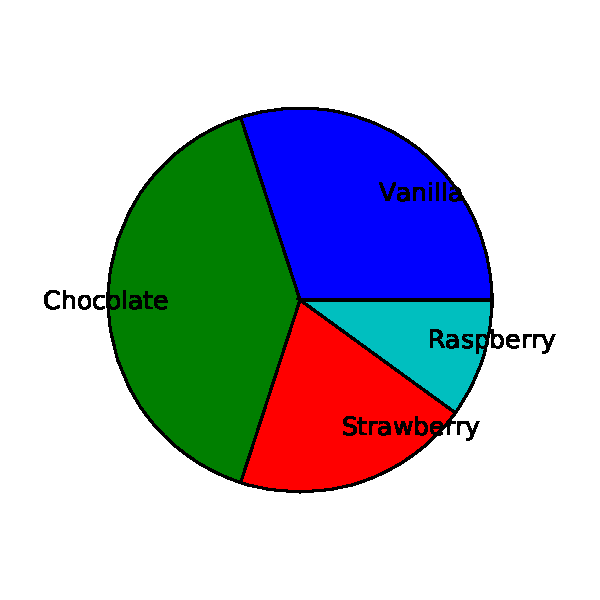
\includegraphics[width=0.6\textwidth]{Chapter-2/figs/pie}
\caption{Here is a sample figure}
\label{fig:hist1}
\end{figure}
%
\begin{figure}[hbtp]
\centering
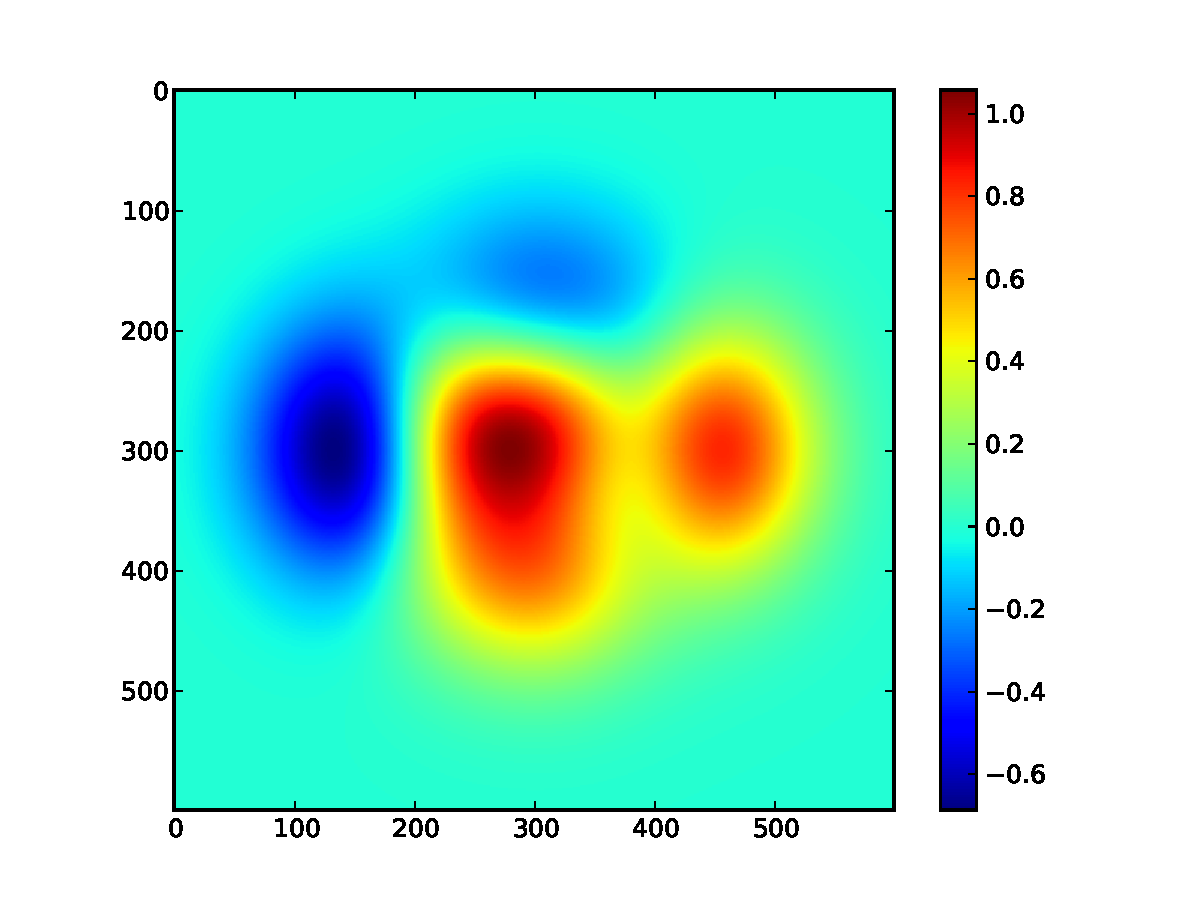
\includegraphics[width=0.6\textwidth]{Chapter-2/figs/color}
\caption{Here is a sample figure}
\label{fig:hist2}
\end{figure}
%
\begin{figure}[hbtp]
\centering
\subfloat[]{
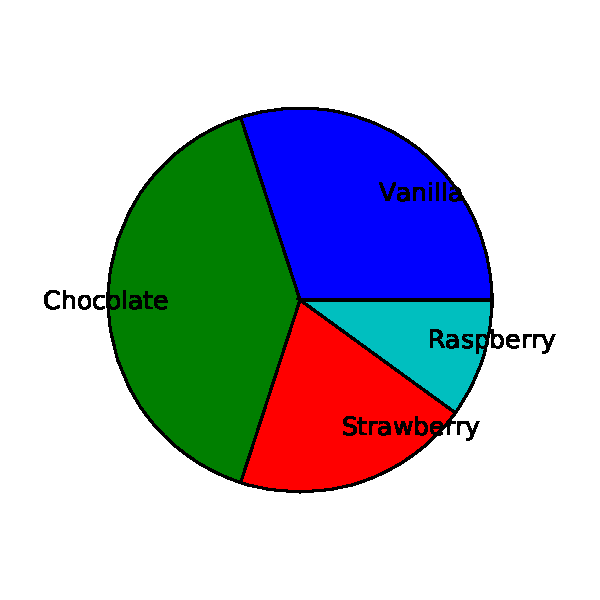
\includegraphics[width=0.4\textwidth]{Chapter-2/figs/pie}
}
\subfloat[]{
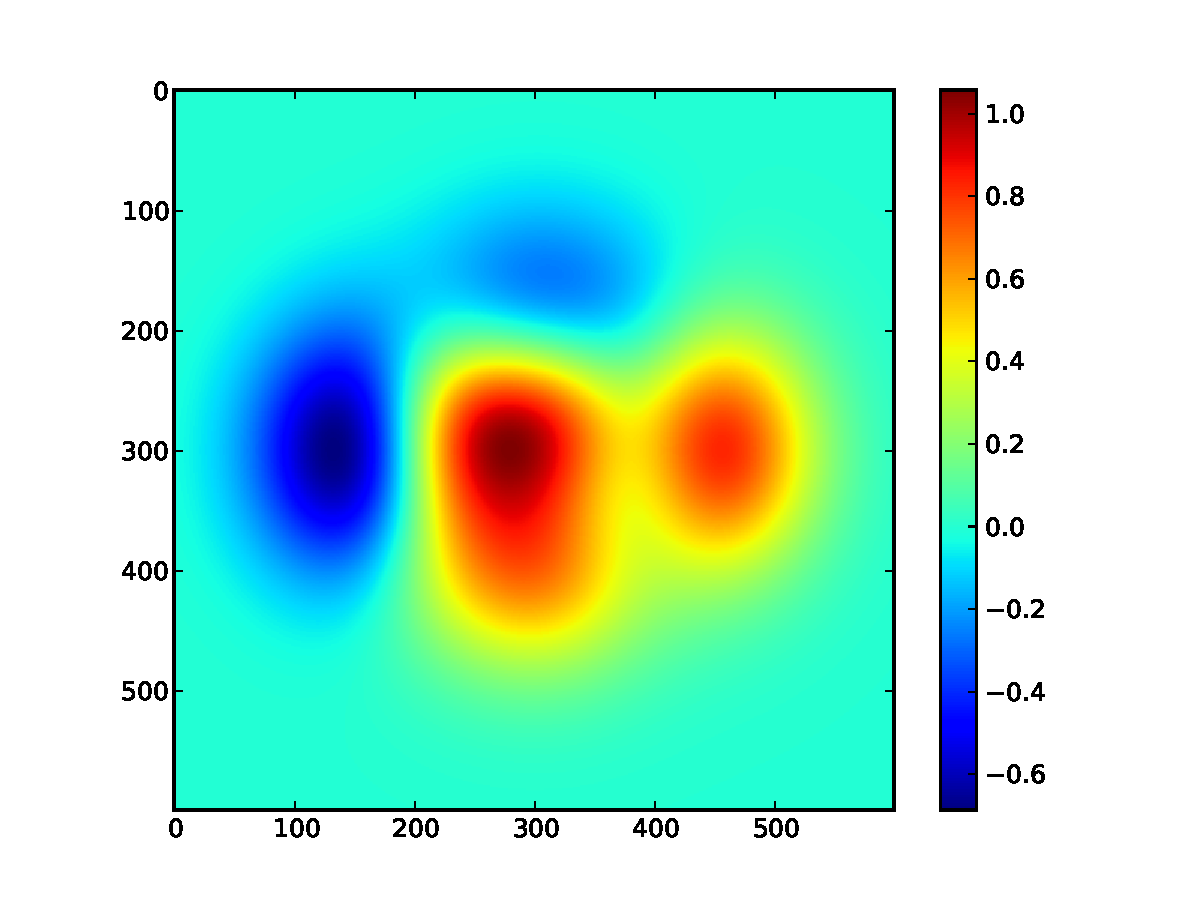
\includegraphics[width=0.4\textwidth]{Chapter-2/figs/color}
}
\caption{Here are two floating subfigures}
\label{fig:subfigures}
\end{figure}


\paragraph{Filler Text} \lipsum[12-15]

\begin{lscape}
\begin{figure}
\centering
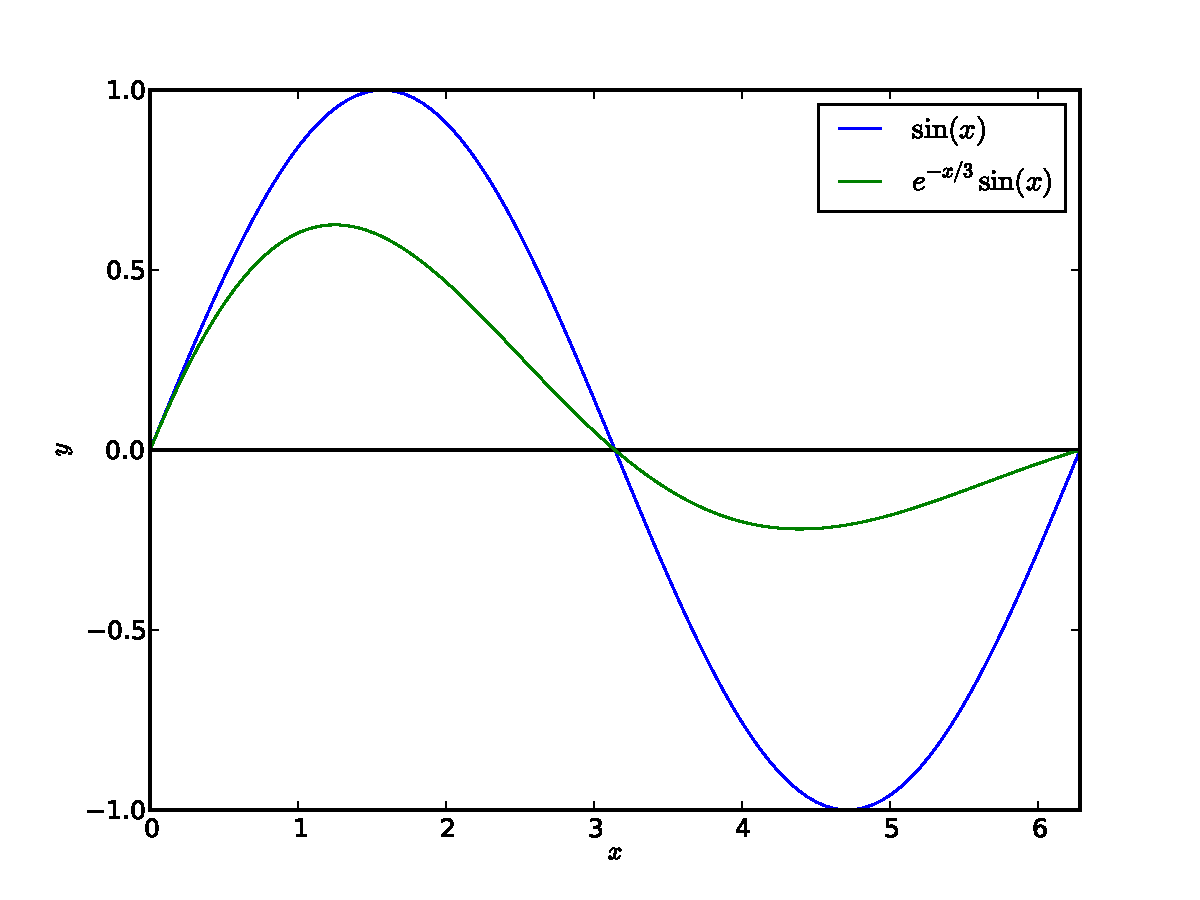
\includegraphics[width=\textwidth]{Chapter-2/figs/sine}
%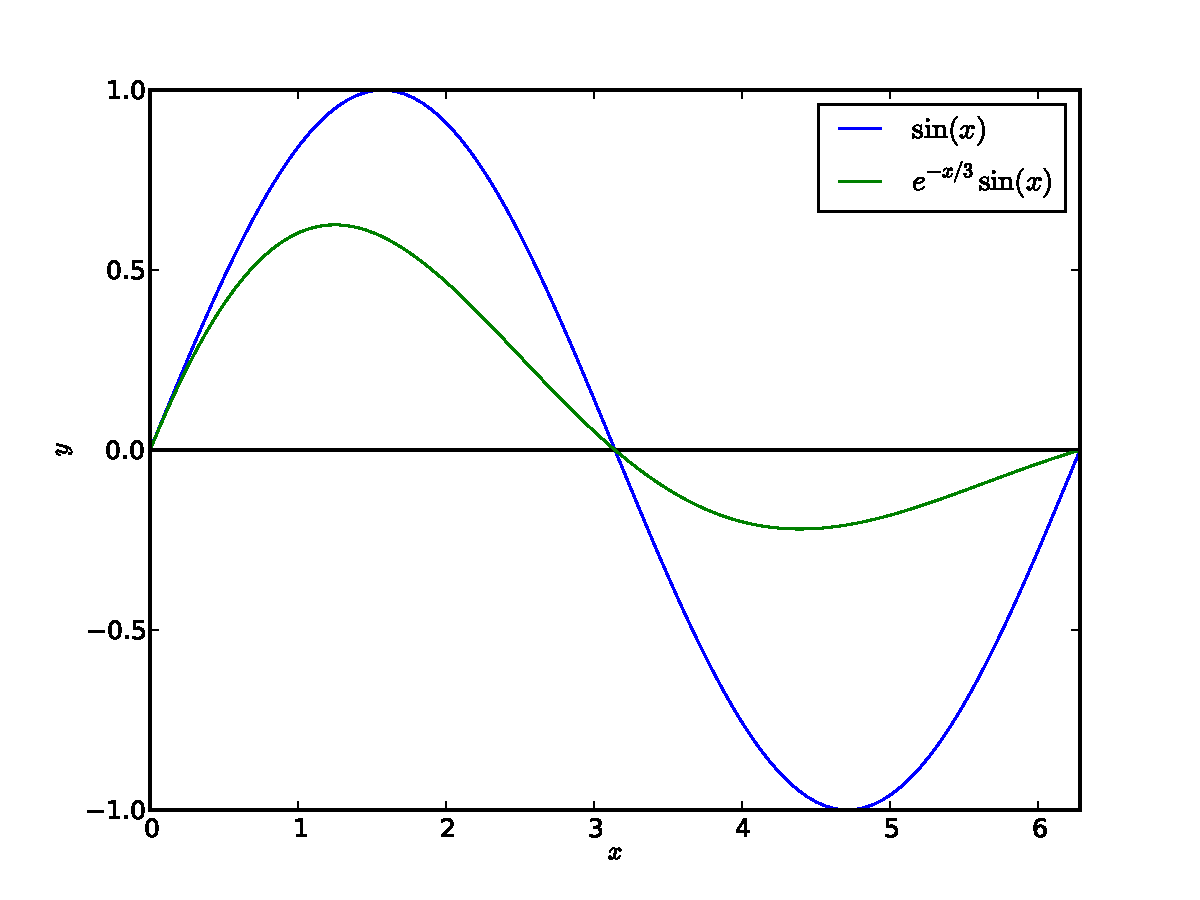
\includegraphics[height=\textwidth]{Chapter-2/figs/sine}
\caption{This figure has been turned sideways.  With large figures, 
         the author must ensure that there are at least two double spaces
         between the caption and the page number.}
\label{fig:hist}
\end{figure}
\end{lscape}

\section{Matrices}
Let's look at a simple example of a matrix:
\[ \left( \begin{array}{ccc}
a & b & c \\
d & e & f \\
g & h & i \end{array} \right)\] 
%
You may prefer to write it this way:
\[ \left[\begin{array} {cccccc}
1 & 0 & 0 & 0 & 0 & 0 \\
0 & 1 & 0 & 0 & 0 & 0 \\
0 & 0 & 1 & 0 & 0 & 0 \\
0 & 0 & 0 & 1 & 0 & 0 \\
0 & 0 & 0 & 0 & 1 & 0 \\
0 & 0 & 0 & 0 & 0 & 1 \\
\end{array} \right] \]

\chapter{Lorem Ipsum}

\section*{A First Section}

\paragraph{Filler Text} \lipsum[1-6]
%
\begin{figure}[t]
  \centering
  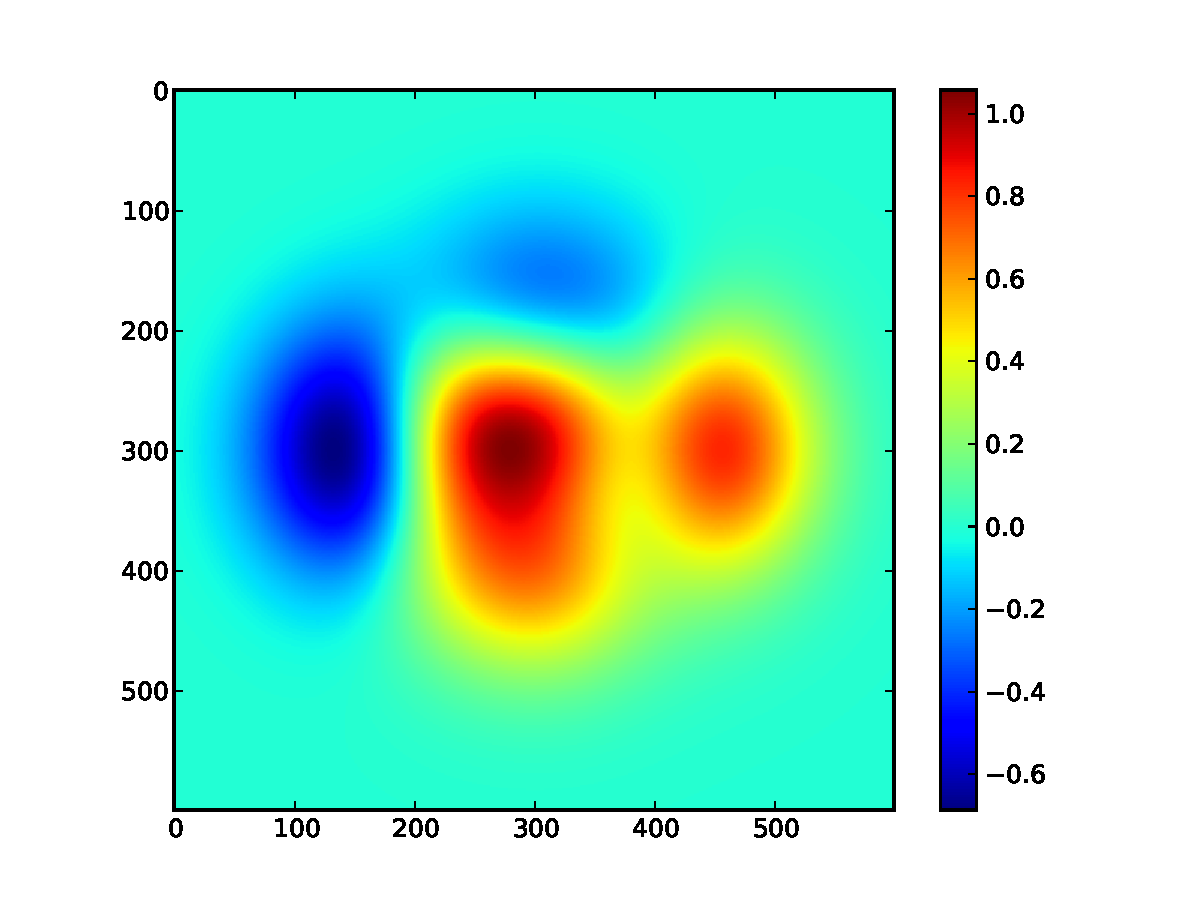
\includegraphics[width=0.6\textwidth]{Chapter-2/figs/color}
  \caption{A figure at the top of the page.}
  \label{fig:ch3.1}
\end{figure}
%
\lipsum[7-13]
%
\begin{figure}[!h]
  \centering
  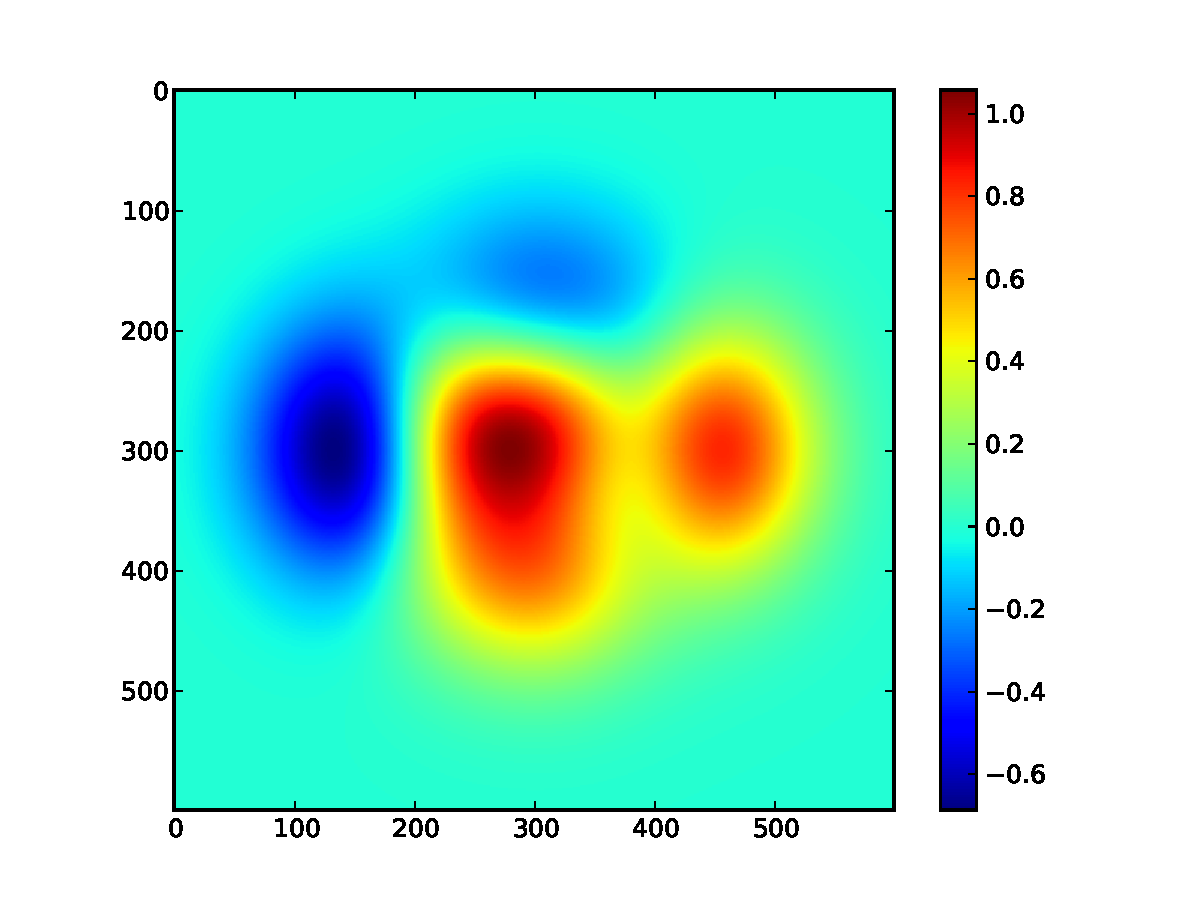
\includegraphics[width=0.6\textwidth]{Chapter-2/figs/color}
  \caption{A figure in the middle of text.}
  \label{fig:ch3.2}
\end{figure}
%
\begin{figure}[!b]
  \centering
  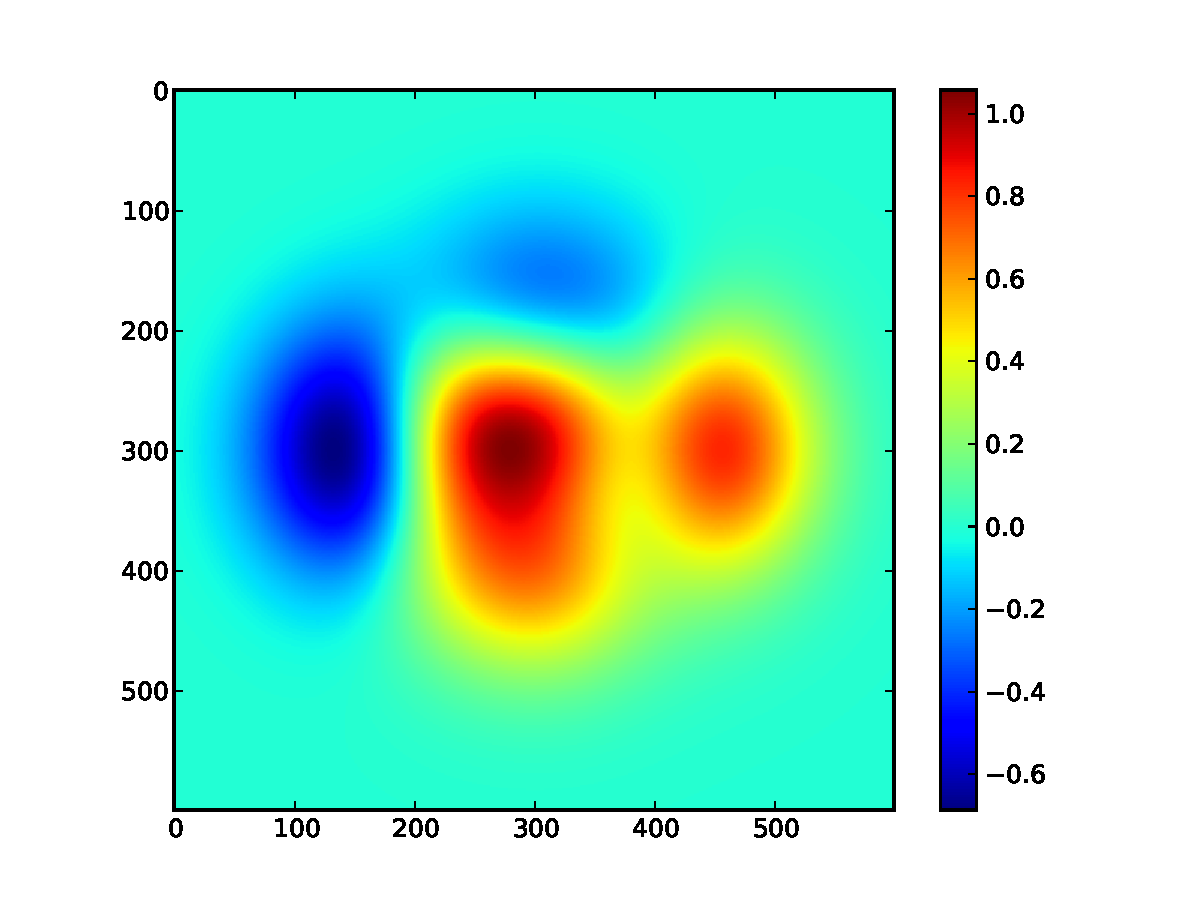
\includegraphics[width=0.6\textwidth]{Chapter-2/figs/color}
  \caption{A figure at the bottom of the page.}
  \label{fig:ch3.3}
\end{figure}
%
\lipsum[14-20]

\chapter{History Reuse Architecture}
\label{chap-four}

\section{Overview}
\label{overview}
For any framework to be successful globally in the computation of History Reuse needed to effectively and comprehensively solve all the challenges motioned above. In addition it also needed to be directly translatable and not be over dependent upon the algorithm in question. Keeping the above framework requirements in mind we finally settle on the framework components as follows:
\subsection{Feature Set Reduction And Normalization}
\label{fet_set_red}
The aim of this section of the framework is to capture the most relevant features of the data set (features along which maximum variation is seen). For this purpose we decided to take a leaf out of the Image processing/statistics books. This step consists of two major parts:
\begin{itemize}
    \item \textbf{Dimension Reduction:} In this part of the algorithm we essentially reduce the total dimensions of the data set to the minimal possible without losing the meaning of the data set. This is achieved by the use of Principal Component Analysis (PCA)\cite{pca}\cite{pca_visual}. PCA is a method, which takes in a data set, and then proceeds to return a modified data set such that the dimensions in the updated normalized data set are arranged in descending order of variance. This way we can take the top few dimensions for our computations.
    \item \textbf{Point Count Reduction:} In this part of the algorithm we essentially aim at selecting the optimal sample set of data-points from the data set for our computations. This is essentially achieved by dividing all the points into buckets. We then proceed to pick the top-k highest populated buckets to get the highest density range of the data set, while at the same time greatly reducing the total no of data-points that needing consideration in our data set.
\end{itemize}
\subsection{Similarity Metric Calculation}
\label{sim_calc}
\begin{itemize}
    \item Once we have evaluated the reduced data-set using steps mentioned in section 5.1, we proceed to calculate the probability based similarity metric. We achieve this using \textbf{\textit{Welch’s Test}}\cite{welch_test} for non-parameterized data for null hypothesis testing. In statistics, Welch's t-test (or unequal variances t-test) is a two-sample location test, and is used to test the hypothesis that two populations have equal means. Welch's t-test is an adaptation of Student's t-test, and is more reliable when the two samples have unequal variances and unequal sample sizes. In our algorithm, we use it to approximate the degree of similarity of means between our current data set and our historic data sets. 
    \item Our assumed null hypothesis for any compared data sets is that both data sets are exactly similar to each other. The Welch test thus gives us a probability metric that states that the difference in data sets is due to chance based on the evaluation of the difference in their means. Thus higher the probability of the difference in data sets being up to chance, the better is the probability that the two sets would be similar. We choose the Welch's test because it gives more accurate results as compared to the Student T-Test for data sets whose distribution in non-Gaussian and whose sample size may be different.
    \item We take individual dimensions from the two data-sets and run Welch Test on them to get a probabilistic measure of their similarity on a per dimension and a cumulative sum across dimensions. We then rank the data sets with respect to each other based on the computed probabilistic metrics. Now this is an important aspect of our computation because this is the algorithm that we used for our probabilistic metric calculation, which is in turn used for ranking all data sets relative to each other.
\end{itemize}
\subsection{History Storage Architecture}
Once we have computed the above-mentioned values for our data set, we store it in memory as objects. Each historical data object holds its original data, PCA metadata (Eigen values and Eigen vectors etc.), bucket-wise histogram and the reduced data set. In addition to this each object also stores a score of the probabilistic similarity it holds with each of the other historical data sets and maintains them in non-increasing order of probability. This is done for quick access of data sets for computations when we are comparing real-time data with historical data sets.
\subsection{Matcher and Selector}
This is by far the most time critical part of the framework. It needs to be quick because this is the function that is responsible for matching the current data set with the sets in the historical data-set and find the best match for computation reuse selection in real-time. Since, historical data may be large, we need a quick way to find the closest match from the historical data set. Our framework goes about doing this in the following two passes:
\begin{itemize}
    \item In the first pass we do the PCA computation for our current set. We then proceed to use the histogram made by the PCA data points for quick distance comparison. We take the highest populated top-k buckets and do a distance computation with points in similar buckets in other data sets. This gives us one candidate for History Reuse. Another candidate is calculated by computing distance as mentioned above but in this case instead of taking highest populated buckets from History Reuse candidates, we now use buckets having closest ranges to the selected buckets for current data set. This is done to estimate similarity in distribution. Doing this we now get another candidate for history reuse. This part of the algorithm runs linearly without much time delay. Thus we can afford to do this kind of matching with all the historical data sets and get the approximate closest match.
    
    \item We now use the above computed candidate historical data sets along with the current data set to compute the probabilistic metric of similarity between the data sets and then proceed to compute the same metric for the top three closest matches to the historical data sets (pre-computed and stored.) We now use the data set with the highest probabilistic similarity to select data set for computation reuse. This step gives us the final candidate for History Reuse.
\end{itemize}

\section{Algorithm: HRu Architecture}
The final algorithm maybe divided into two major categories: Training and Run Time. 
\begin{itemize}
	\item \textbf{Training Algorithm}: The training algorithm is used to prepare and store data so as to have highest availability of reuse components for all candidates. This part of the algorithm is carried out offline and thus does not affect the run time of the algorithm when run for most current data set.
	\item \textbf{Run Time Algorithm:} The run time algorithm is responsible for choosing the best match historical data set to be used for Computation Reuse. This part of the algorithm is online, thus it has a direct impact on the run time for the algorithm when run for current data set. This part of the algorithm must be quick and must ensure that the computation time required for historical data set selection not overshoot the time for benefits gained by such history reuse.
\end{itemize}

Both the training algorithm and the run time algorithm use some complex methodologies to ensure the best possible approach for historical data set selection. These are defined in the following sub sections.

\subsection{Principal Component Analysis (PCA)}
\label{principal_comp_analysis}
	PCA\cite{pca}\cite{opencv_library} \cite{opencv_manual} and project data set points on thus computed Eigen vectors. PCA essentially extracts the top \textit{n} most influential \textit{features} of a data set. For our algorithm we choose the \textbf{top 3 principal components.} PCA returns Eigen vectors for the three chosen principal axis (or components) for our data set based on maximum variance for each feature set (represented by a single column). We then proceed to project the data onto the new Eigen plane using the above computed Eigen vectors. This step reduces the dimensionality of our data into a fixed three-dimension space.
\textbf{figure}  \ref{subfig:pca_real_data} shows an example data distribution in a 2-D plane and \textbf{figure} \ref{subfig:pca_proj_data} shows the same data projected into a 2-D Eigen plane. Since Eigen planes are always coplanar, this thus normalizes the data along the same axes. 

\begin{figure}[!ht]
	\centering
    \subfloat[Example: Real Data with 2 Dimensions\label{subfig:pca_real_data}]{%
      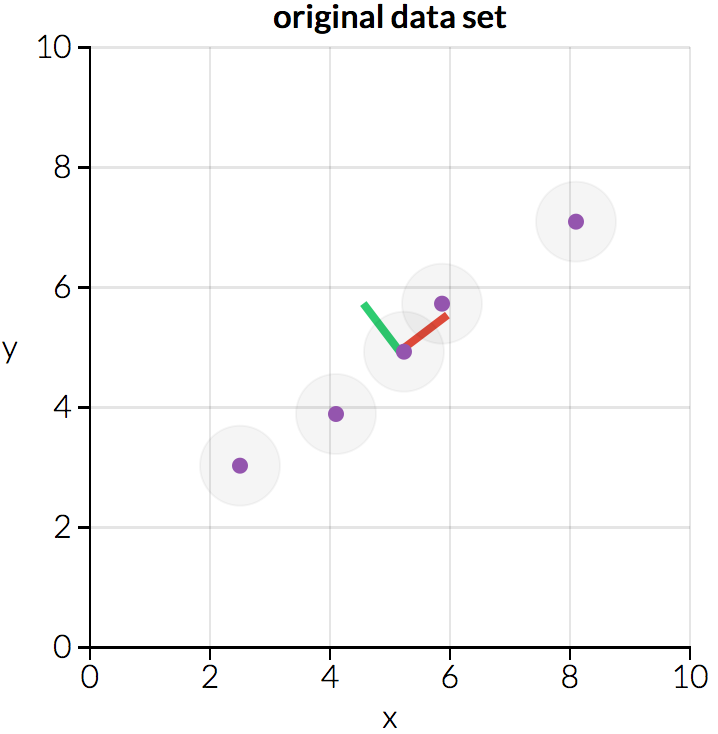
\includegraphics[width=0.45\textwidth]{Chapter-4/figs/pca_real_data}
    }
    \hfill
    \subfloat[Example: Data Projected on Eigen Plane\label{subfig:pca_proj_data}]{%
      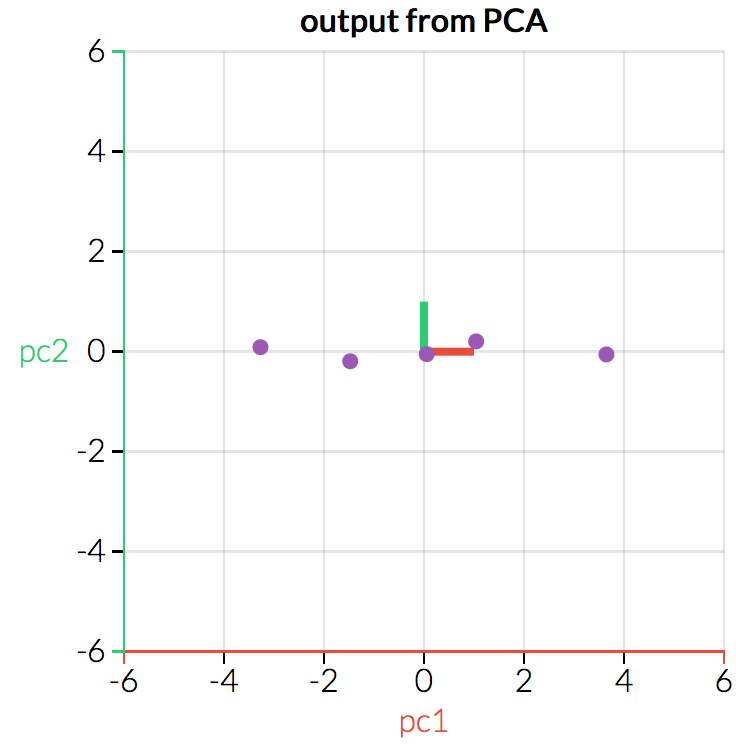
\includegraphics[width=0.45\textwidth]{Chapter-4/figs/pca_proj_data}
    }
    \caption{PCA Projection Example}\cite{pca_visual}
   \label{fig:pca_prog_eg}
 \end{figure}
  
  We can also see from figure \ref{subfig:pca_proj_data} that maximum variance of data is along the \textbf{pc1 axis}. This makes the \textbf{pc1 axis} the 1st principal component of the data. Using this property of PCA we can choose the most important \textit{features} only from a data set while excluding the less important \textit{features}. We see from \textbf{figure} \ref{pca_real_data_on_axis}, real data needs both the \textbf{x and y plane} to represent the features (spread) of the data. On the other hand in \textbf{figure} \ref{pca_proj_data_on_axis} we can see that most of the variance for the data items has been condensed with negligible variance along the \textbf{pc2 axis}. All features of the data can now be abstracted onto the \textbf{pc1} plane. This method is the method we use for data abstraction while maintaining the features of the data set.% \ref{fig:pca_feature_set_abstraction} \ref{pca_proj_data_on_axis} \ref{pca_real_data_on_axis}
 
 \begin{figure}[!ht]
	\centering
    \subfloat[Example: Variance for Real Data on X and Y axis individually\label{pca_real_data_on_axis}]{%
      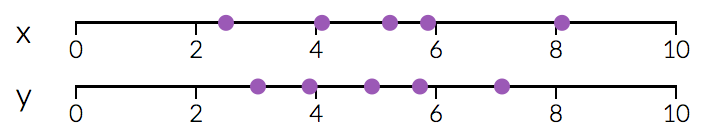
\includegraphics[width=0.45\textwidth]{Chapter-4/figs/pca_real_data_axis}
    }
    \hfill
    \subfloat[Example: Variance of Data on PCA axis individually\label{pca_proj_data_on_axis}]{%
      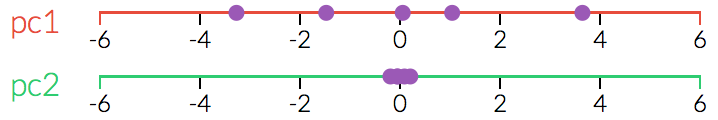
\includegraphics[width=0.45\textwidth]{Chapter-4/figs/pca_proj_data_axis}
    }
    \caption{Feature Set Abstraction}
   \label{fig:pca_feature_set_abstraction}
 \end{figure}
  
\subsection{Histogram Generation}
\label{hist_generation}
  Once the dimensionality of the data has been reduced using PCA, we need to reduce the point count ensuring we use the most dense distribution areas for data set comparisons. We tackle this problem by the use of Histograms.
Histogram is then generate on a per dimension \textit{(di)} basis with each dimension having 16 or 32 buckets with ranges computed as follows : 
\begin{equation}
     \begin{aligned}
       & bucket\_count = 16 \ or \  32 \\
       & dim\_bucket\_range_{di}\  =\  max_{di} \   - \   min_{di}: \  \forall\  di\  in\  (1\   ..\   3) \\
       & bucket\_size_{di} \   = \   dim\_bucket\_range_{di} \   / \    bucket\_count \ : \  \forall\  di\  in\  (1\   ..\   3) \\
       &  bucket\_range_j = [(bucket\_size * bucket_j + min_{di}), (bucketSize * (bucket_j + 1) + min_{di})); \\  
       & \forall \ j \ in \ (1\ .. \ n)
     \end{aligned}
\end{equation}

This will give us the buckets with their ranges for all dimensions. We then proceed to generate \textit{three} histograms. Each data point is put into a bucket based on its value for that particular dimension. 
\textit{E.g.:} let \textit{three points} be represented in a 3-D Eigen plane by coordinates as follows: \\
$p1 = (1,\ 2,\ 3)$
$p2 = (-1,\ 0,\ 1)$
$p3 = (2,\ 3,\ 4)$ \\ 
Now, let there exist 2 buckets per dimension with Ranges as follows:  \\
$b_{11} = [-1,\ 2)$
$b_{12} = [2,\ 4)$
$b_{21} = [0, \ 2)$
$b_{22} = [2, \ 4)$
$b_{31} = [1, \ 3)$
$b_{32} = [3, \ 5)$ \\

Using the above points and bucket ranges we will now generate \textbf{3 Histograms}(one per dimension) with \textbf{2 buckets per histogram.} The histograms may be represented as follows: \\
$h\_points_1\ =\ {b_{11}\ :\  (p1,\  p2);\ b_{12}\ :\  (p3)\ };\ \text{Histogram for first dimension}$\\
$h\_points_2\ =\ {b_{21}\ :\  (p2);\ b_{22}\ :\  (p1, \ p3)\ };\ \text{Histogram for second dimension}$\\
$h\_points_3\ =  {b_{31}\ :\  (p2);\ b_{32}\ :\  (p1, \ p3)\ };\ \text{Histogram for third dimension}$\\

Thus we can see from above example how each item becomes a part of a bucket if its coordinate for the given dimension lies in the bucket range for that dimension.

\subsection{Similarity Metric Computation}
\label{similarity_metric_calculation}
We now use the Welch's Test \cite{welch_test}\cite{boost_graph} to compute the probabilistic metric for similarity and to rank all history data sets wrt to each other and store in decreasing order of similarity. (Note: Will be used in run time historical reuse data set computation.) 
Welch test is computed for each dimension of the two sets being matched and the summation of the score for all three dimensions is as Similarity score for the two data set. Data sets are then ranked with each other based on the similarity score. Higher score means a better and match and vice versa.
\subsection{Training Algorithm}
This part of the algorithm is used to prepare and store data so as to have highest availability of reuse components for all candidates. We try and solve the challenges mentioned in \autoref{chap-three} using the methods mentioned in \ref{overview}. 
Let our history database consist of "n" data sets named: $HD_1, HD_2, ... HD_n$.
The following Steps are done for each $HD_i \text{  for (i in 1 to n) } $:
\begin{itemize}
    \item \label{pca_gen_training} \textbf{PCA:} Compute Eigen vectors for $HD_i$ and project data on the Eigen vectors to normalize in Eigen plane and reduce dimensionality as shown in \ref{principal_comp_analysis}. We reduce all data into 3-D space for comparison purposes.
    \item \label{his_gen_training} \textbf{Histogram Generation:} Categorize PCA data for $HD_i$ buckets for histograms as shown in \ref{hist_generation}. One histogram is generated per dimension of data, thus we have a total of 3 histograms for each data set. Each histogram comprises of a total of 32 buckets. 
    \item \textbf{Relative Ranking:} Use Welch Test to rank all history data sets wrt to each other. Data sets are stored in decreasing order of similarity as shown in Algorithm \ref{hist_relative_ranking}. (Note: Will be used in run time historical reuse data set computation.)
    \item \textbf{Reuse Data for Data Set:} Run Algorithm of choice for Data Set and store \textit{Computation Reuse Data}. E.g.: In case of the K-means algorithm we choose the \textit{final centroids} computed by the K-Means Algorithm for current data set.
\end{itemize}


%==================================================================
%			History Rank ALGORITHM	BEGIN
% ==================================================================
\begin{algorithm}
\caption{History Data Sets- Relative Ranking}
\label{hist_relative_ranking}
\begin{algorithmic}[1]
\Procedure{RankHistoryData}{$History\_Database$}
\State $relative\_rank_{map}\ =\ ORDERED\_MAP(Similarity\_Score,\ Data\_Set)$
\State $score_{Final} = 0$
\For{each $HD_i$ in $History\_Database$}
	\For{each $HD_j$ in $History\_Database$ != $HD_i$}
		\State $score_{Final}$ = $ComputeSimilarity(HD_i,\ HD_j)$
		\State $relative\_rank_{map}.insert(score_{Final},\ HD_j)$
	\EndFor
	\State$(HD_i).Relative\_Ranking$ = $relative\_rank_{map}$
\EndFor
\EndProcedure
\end{algorithmic}
\end{algorithm}

%==================================================================
%			History Rank ALGORITHM	BEGIN
% ==================================================================

%==================================================================
%			Welch ALGORITHM	BEGIN
% ==================================================================
\begin{algorithm}
\caption{Similarity Metric Computation}
\label{similarity_computation}
\fontsize{10}{15}
\begin{algorithmic}[1]
\Procedure{ComputeSimilarity}{$Data\_Set_{Current},\  Data\_Set_{Historic}$}
\State $score_{Final} = 0$
\State $Data_{CurDS} = TOP\_THREE\_BUCKET\_DATA(Data\_Set_{Current})$
\State $Data_{HistDS} = TOP\_THREE\_BUCKET\_DATA(Data\_Set_{Historic})$
\For{each $dim_i$ in $Dimensions(Data\_Set_{Current})$}
	\State $score_{Final}$ += $CalcWelchScr(Data_{CurDS}.columnAt(dim_i),\ Data_{HistDS}.columnAt(dim_i))$
\EndFor
\State\Return $score_{Final}$
\EndProcedure
\end{algorithmic}
\end{algorithm}

%==================================================================
%			SCREENING ALGORITHM	BEGIN
% ==================================================================

 
\begin{algorithm}
\caption{Screening Algorithm}
\label{screening_algo}
\begin{algorithmic}[1]
\Procedure{Screening\textendash PrimaryCandidateSelection}{}
\State $least\_distance_{rank} = MAX$
\State $least\_distance_{range} = MAX$
\State $dim\_distance_{rank} = 0$
\State $dim\_distance_{range} = 0$
\State $HD\_Rank_{selected}$
\State $HD\_Range_{selected}$
\For {each $HD_x$ in History Database} 
	\For { each $Dim_i\  where\ i\  in\  1\  ..\  3\ $ }
		\For{each  $Bucket_j$ in Top 3 Buckets($Dim_i$) in Decreasing Order of Item Count for current data set} 
			\State 
			\For{each  $pt_{cd}$ and $pt_{HDi}$ in points($Bucket_j$)} 
				\State $distance_{rank}\ =\  dist(pt_{cd},\ pt_{HDi})$;
			\EndFor

			\State$Bucket_k$ = Bucket in $HD_i\  where\ range(bucket_k)\ \sim \  range(bucket_j)$
			
 	 		\For {each  $pt_{cd}\  in\ points(Bucket_j)\ and\ pt_{HDi}\ in\ Bucket_k$ } 
				\State $distance_{range}\ =\ dist(pt_{cd},\ pt_{HDi})$;  
			\EndFor
		\EndFor
 	 		
		\State $dim\_distance_{rank}\  =\  dim\_distance_{rank} \ + \ distance_{rank}$
		\State $dim\_distance_{range}\  =\  dim\_distance_{range} \ + \ distance_{range}$ 
	\EndFor
	\If{$dim\_distance_{rank}$ < $least\_distance_{rank}$}
 			\State $least\_distance_{rank}$ = $dim\_distance_{rank}$;
			\State $HD\_Rank_{selected}\ = \ HD_x$;
	\EndIf
   	 
	\If{$dim\_distance_{range}$ < $least\_distance_{range}$}
   		\State $least\_distance_{range}\ = dim\_distance_{range}$;
   	 	\State $HD\_Range_{selected}\ = \ HD_x$;
	\EndIf
\EndFor
\State\Return [$HD\_Rank_{selected}$, $HD\_Range_{selected}$]
\EndProcedure
\end{algorithmic}
\end{algorithm}


%==================================================================
%			SCREENING ALGORITHM	END
% %================================================================

%==================================================================
%			Best Match Computation ALGORITHM	BEGIN
% ==================================================================
 
\begin{algorithm}
\caption{Best Match Selection Algorithm}
\label{best_match_selection}
\fontsize{10}{15}
\begin{algorithmic}[1]
\Procedure{BestMatchSelection}{}
\State $primary\_candidates = Screening$\textendash$PrimaryCandidateSelection$
\State $best\_match\_score_{final} = INT_MIN$
\State $best\_match\_score_{cur}$ = $ComputeSimilarity(Data\_Set_{current},\ primary\_candidates[0])$
\State $best\_match_{data\_set} = primary\_candidates[0]$
\State $best\_match\_score_{cur}= ComputeSimilarity(Data\_Set_{current},\ primary\_candidates[1])$
\If{$best\_match\_score_{cur}$ > $best\_match\_score_{final}$}
	\State $best\_match\_score_{final} = best\_match\_score_{cur}$
	\State $best\_match_{data\_set} = primary\_candidate[1]$
\EndIf
\For {each $HD_x$ in $TOP\_THREE{relative_rank}$($primary\_candidates[0]$)} 
	\State $best\_match\_score_{cur} = ComputeSimilarity(Data\_Set_{current},\ HD_x)$
	\If{$best\_match\_score_{current}$ > $best\_match\_score_{final}$}
		\State $best\_match\_score_{final} = best\_match\_score_{cur}$
		\State $best\_match_{data\_set} = HD_x$
	\EndIf
\EndFor

\For {each $HD_y$ in $TOP\_TWO_{relative_rank}$($primary\_candidates[1]$)} 
	\State $best\_match\_score_{cur} = ComputeSimilarity(Data\_Set_{current},\ HD_y)$
	\If{$best\_match\_score_{cur}$ > $best\_match\_score_{final}$}
		\State $best\_match\_score_{final} = best\_match\_score_{cur}$
		\State $best\_match_{data\_set} = HD_y$
	\EndIf
\EndFor
\Return  $best\_match_{data_set}$
\EndProcedure
\end{algorithmic}
\end{algorithm}

%==================================================================
%			Best Match Computation ALGORITHM	END
% %================================================================


\subsection{Computing Best Match for Current Data-set (Run Time)}
This is the part of the algorithm that is actually responsible for the selection of the 
\begin{itemize}
	\item \textbf{PCA:}  Compute PCA for current Data Set similar to \ref{pca_gen_training}.
	\item \textbf{Histogram Generation:} We again characterize PCA data into 3 histograms with 32 buckets each as done in \ref{his_gen_training}.
	\item \textbf{Matcher and Selector :}The best match data set selection process is divided into 2 parts: screening and final selection. Screening is used to prune our Historical Data Sets to a smaller subset from which we can select our best match Data Set for computation reuse using the final selection step.
	
	The two parts of the Matcher and Selector part of our algorithm may be defined as follows:
	\begin{itemize}
	\item \textbf{Screening:} This is the process where we select our initial candidates for the next step of our selection algorithm. This part of the algorithm essentially estimates the similarity in distribution for the current and corresponding historical data sets using the  Histograms generated in the previous steps. Variance Similarity is estimated as follows:			
		\begin{enumerate}
    			\item Take top-k most populated buckets for current data set and select corresponding top-k bins from all history data sets and top-k buckets with closest min and max to current data-set top-k bins.
		    \item Find ED for these data points between current data set and all historical data sets.
    			\item Choose Historical Data Sets with minimal distance as initial “Best Match” for both top-k buckets by rank and top-k buckets by range.
		\end{enumerate}
	Pseudo Code for an understanding of how our \textit{screening algorithm} runs can be seen in Algorithm \ref{screening_algo}.
	\item \textbf{Find Best Match (Similarity Metric => Probabilistic Score):} 
	One we have found the best match candidates from out screening step, we simple calculate the Welch Test score for each dimension ($dim_i$) for each pair of current data set and chosen historic data sets.
		\begin{enumerate}
    			\item Find ``Similarity Metric`` as expalined in subsection \ref{sim_calc} and between current data set and above chosen “best match” data sets using Welch’s Test for all dimensions of all three data sets as shown in Algorithm \ref{similarity_computation}.
		    \item Similarly find “Similarity Metric” for top two relatively ranked data sets for current best match and top one for second best match.
		    \item Choose Data Set with highest Probability Score.
		\end{enumerate}
			Pseudo Code for an understanding of how our \textit{final selection algorithm} runs can be seen in Algorithm \ref{screening_algo}.
	\end{itemize}		
	\item \textbf{Reuse Computations: }  In this section we use the computational data we had stored for history reuse in the training run for the historical data set selected. For instance, in the case of the K-Means algorithm, we now use the centroids from the chosen historical data set that were computed during the training run for historical data.
\end{itemize}
\section{Discussion}
Our final algorithm was reached at after a fair few trials and errors. Some of the major approaches used apart the latest approach for major challenges may be defined as below:
\subsection{Computation on Real Data and Incorrect Screening algorithm:}
\subsubsection{Implementation}
\begin{itemize}
    \item In this method I had initially use bin wise reduction on initial (real) data and then used PCA for dimension reduction of these reduced data points for the calculation of Eigen vectors and Eigen values only.
    \item I had then proceeded to run Student’s T-Test for relative ranking in training Run on real data.
    \item For Run Time computation I had used only the distance between the Eigen vectors for initial screening, choosing the data set with smallest difference in Eigen vectors as initial Best Match data set.
    \item I had then proceeded to Use Student T-Test on real data for computation of the probabilistic metric using all dimensions for the computation of the same.
    \item Python Numpy Libraries had been used for Student T-Test computation.
    \item History Reuse component Computations during training run was done on real data of historical data set instead of PCA data.
\end{itemize}
\subsubsection{Reasons for failure}
\begin{itemize}
    \item Data was not normalized thus computation would not be correct.
    \item Student T-Test worked only with Gaussian Distributions. Garbage value was returned for non Gaussian Data.
    \item Eigen Vectors of two data set may be orthogonal yet PDF (probability density function) may be close enough such as to generate similar clusters.
    \item Use of labels for direct initialization was flawed in the sense that if the data points were jumbled they would produce the wrong order of labels thus still providing a bad match.
    \item Bin Wise distribution of data points was an expensive operation and computation overhead increased with increase in dimensionality of data.
    \item Student T-Test had to compute for multiple dimensions of data and was a time expensive computation.
\end{itemize}
\subsection{Custom CPP Implementation for Welch’s Test}
Some of the earlier seen issues were corrected in this section as I noticed that a lot of the run time improvement was overshadowed by the time taken for choosing the historical data set. I also noticed that the Student T-Test was not reliable for non-Gaussian data and failed completely in case of different data set sizes.
This iteration was also mainly about ensuring quicker run time for the selection algorithm, so incremental updates were made to optimize the same. Some of the updates made may be enlisted as follows:
\begin{itemize}
    \item Implemented Custom Cpp implementation for Welch’s Test to over come overhead created by using python libraries for it and calling python script from Cpp.
    \item Removed the distribution of data into bins for data point reduction as it had a big overhead in computation and CPP Welch Test Libraries scaled well for larger data sets.
    \item Changed to use of Welch’s Test as compared to Student T-Test as Welch’s Test works with non Gaussian distributed data as well as compared to Student T-Test which makes assumptions of data distribution being Gaussian in nature.
    \item For Run Time computation I had used only the distance between the Eigen vectors for initial screening, choosing the data set with smallest difference in Eigen vectors as initial Best Match data set.
    \item Centroid Computation during training run was done on real data of historical data set instead of PCA data.
    \item Labels for Best Match historic data set were used as-is for current data set.
\end{itemize}
\subsection{Random Sampling for Order comparison.}
Experimentation on the approach showed non-reliable best match selection. Also I saw that often the best match might not even yield best results. One of the major reasons for this was the use of the incorrect use of historical data. For instance, in case of the K-Means algorithm the use of labels instead of the computed centroids lead to dependence on the order of the items in the historic data set. While the two data set may be similar and produce similar clusters, History Reuse with this method would still fail as initially the data points in current data set may get labeled incorrectly. I also realized that comparison of non-normalized data was in its very essence. I tried to correct the above issues with the following methodology:
\begin{itemize}
    \item Changed implementation to use of PCA data for most computations.
    \item Projected Historical data set points on Current Data Set Eigen Vectors. Used distance between data points of Current Data Set and historical data sets by randomly sampling 10\% of data sets against each other. Chose Data Set with minimum distance. This was done to try to use Historical data set with most point order similarity (and thus generated label order similarity) in conjunction with overall data set similarity.
    \item Welch’s Test was still used across all dimensions of actual data Similarity Metric Computation.
    \item Labels were used as-is for real data.
\end{itemize}
This implementation though corrected some of the above mentioned issues, it in its turn generated new issues:
\begin{itemize}
    \item Use of labels for direct initialization was flawed in the sense that if the data points were jumbled they would produce the wrong order of labels thus still providing a bad match.
    \item Random Sampling was a bad way to judge the order of the labels that would be generated by K-Means for data set.
    \item Eigen Vectors of two data set may be orthogonal yet PDF may be close enough such as to generate similar clusters.
\end{itemize}
\subsection{Use Of PCA Data for Welch’s Test and PCA data for centroid computation in Training Run:}
Experimentation still showed both the history reuse to be inconsistent and the overhead of computing historical data set was still quite large. I also realized that while Eigen Vectors of two data set may be orthogonal yet PDF might be close enough such as to generate similar clusters. To correct the above issues I used the following methods:
\begin{itemize}
    \item Used PCA data in training run for Centroid computation of historical data.
    \item Used PCA data for Welch’s Test based “Similarity Metric” computation.
    \item Still used labels from best match historical data set as initialization for current data set.
    \item Stopped projecting historical data sets data on current data set Eigen vectors, instead used self-projection, which could be done offline.
    \item Used Random Sampling for initial estimation of best match data set.
\end{itemize}
The use of Labels was still flawed. Also the use of random sampling was not a very effective methodology for screening as it would often lead to the selection of bad candidates.



\chapter{Evaluations}
\label{chap-five}

\section{Methodology}
We have used leave-one cross testing for all experimentations. Most data sets for experimentation are stock databases available on the UCI machine-learning repository while some source data sets are Microsoft released source data sets for machine learning.
These data sources are then divided into data sets. Depending on the size of the data source\cite{uci_machine_repo} we may have any where between 10 to 43 data sets, where in all save one are treated as historic data sets. We have also allowed all algorithms to converge to the same epsilon error rate thus ensuring the run time comparison for similar quality output for algorithms.
All experiments have been carried out on Octa core Intel Xeon CPU E5-2650 Running Ubuntu Linux 14.04 LTS with 16GB of RAM.
\section{Experiments}
To demonstrate the efficacy and efficiency of our program we evaluate our approach by testing it on various large real world data-sets and compare our algorithm to two most frequently used and vastly accepted K-Means initialization algorithms: standard K-Means (Random Select initialization also known as Lloyd's Algorithm) and K-Means++ initialization (Weighed Probability based initialization based on squared of distance from initial randomly selected center). Both the above algorithms are implemented in the OpenCV library, which has been used as the standard library for Lloyd’s Algorithm implementation. We run all three algorithms on the same data sets with the same error rate for convergence.
We have also compared the historical data-set selected by our algorithm to all other data-sets available in history to show the accuracy of our algorithm in selecting the best available data-set.

\begin{figure}[h!]
    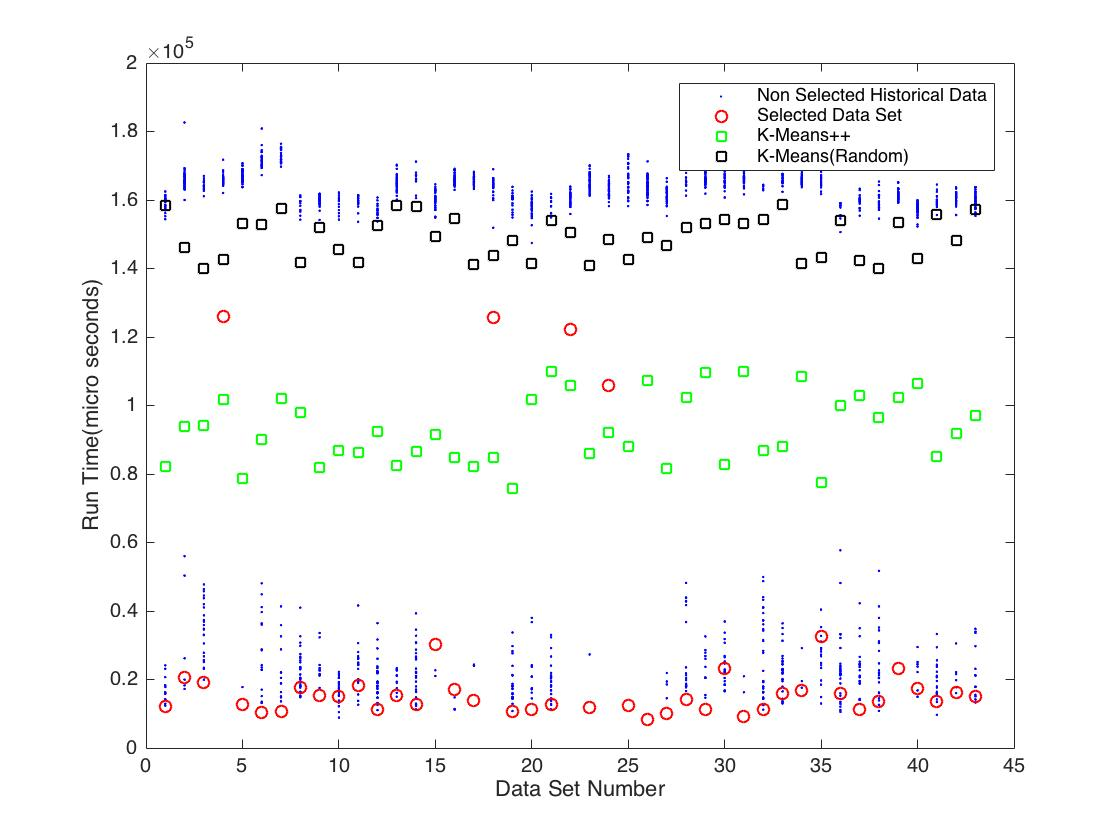
\includegraphics[width=\textwidth]{Chapter-5/figs/road_240}
    \caption{Hit-Rate (Road Network k=120)}
    \centering
    \label{fig:gas_240_selection}
\end{figure}

\begin{figure}[t!]
    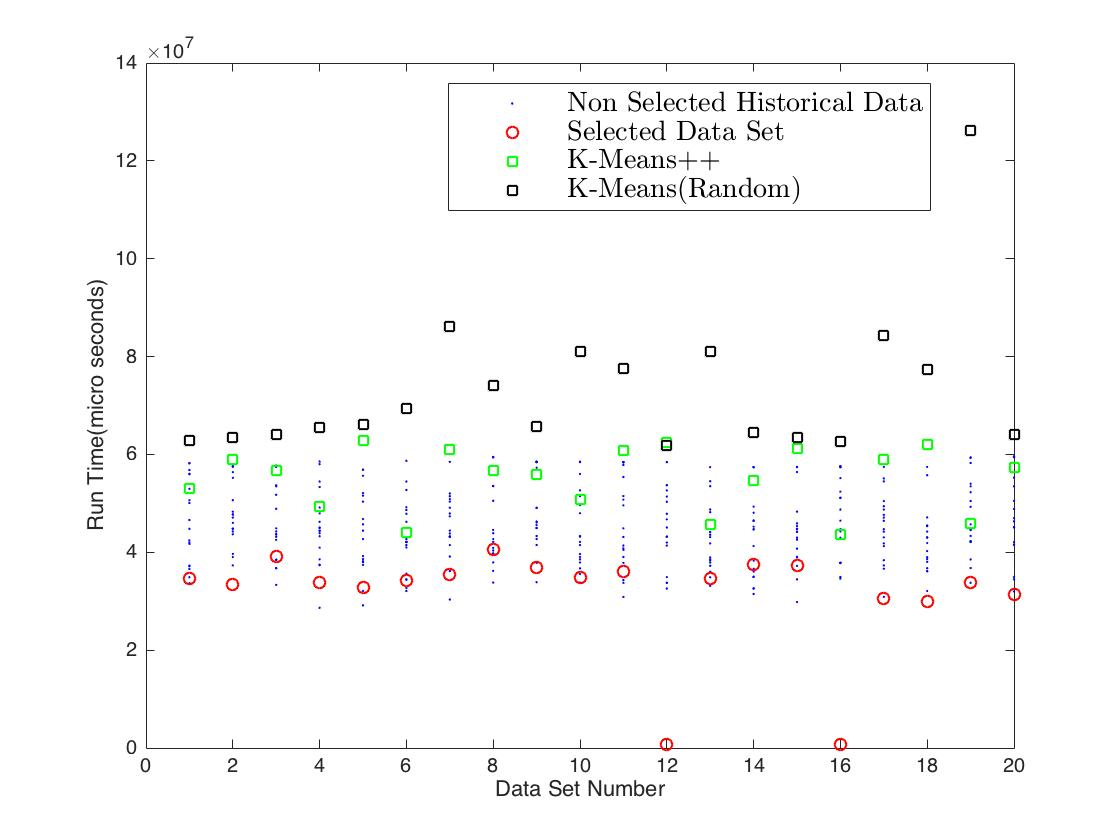
\includegraphics[width=\textwidth]{Chapter-5/figs/nnData_600}
    \caption{Hit-Rate (Caltec 101 for k=600)}
    \centering
    \label{fig:caltec_600_selection}
\end{figure}

\setlength{\arrayrulewidth}{0.2mm}
\setlength{\tabcolsep}{10pt}
%\renewcommand{\arraystretch}{1}
\begin{table*}[h!]
% \begin{minipage}{\textwidth}
\centering
% \begin{center}
\begin{tabular}{|l|c|c|c|r|}
\hline\hline
    \textbf{Data-set Name} & \textbf{History Data-set cnt.} & \textbf{Cluster Count} & \textbf{Top 5 cnt} & \textbf{Hit Rate \%} \\
\hline\hline
    \textbf{Road Network}   & 43 &
    \begin{tabular}{c} 40 \\ 80 \\ 120 \\ 240 \end{tabular} &
    \begin{tabular}{c} 42 \\ 41 \\ 43 \\ 43 \end{tabular} &
    \begin{tabular}{c} 97.67\% \\ 95.34\% \\ 100\% \\ 100\% \end{tabular} \\
\hline
    \textbf{Kegg Network}   & 10 &
    \begin{tabular}{c} 40 \\ 80 \\ 120 \\ 240 \end{tabular} &
    \begin{tabular}{c} 8 \\ 9 \\ 8 \\ 8 \end{tabular} &
    \begin{tabular}{c} 80\% \\ 90\% \\ 80\% \\ 80\% \end{tabular} \\
\hline
    \textbf{US Gas Sensor Data}   & 36 &
    \begin{tabular}{c} 40 \\ 80 \\ 120 \\ 240 \end{tabular} &
    \begin{tabular}{c} 28 \\ 29 \\ 29 \\ 28 \end{tabular} &
    \begin{tabular}{c} 77.7\% \\ 80.5\% \\ 80.5\% \\ 77.7\% \end{tabular} \\
\hline
    \textbf{NotreDame}   & 20 &
    \begin{tabular}{c} 40 \\ 80 \\ 120 \\ 240 \end{tabular} &
    \begin{tabular}{c} 17 \\ 18 \\ 17 \\ 17 \end{tabular} &
    \begin{tabular}{c} 85\% \\ 90\% \\ 85\% \\ 85\% \end{tabular} \\
\hline
    \textbf{Tiny}   & 20 &
    \begin{tabular}{c} 80 \\ 120 \\ 240 \\ 360 \\ 480 \\ 600 \end{tabular} &
    \begin{tabular}{c} 20 \\ 18 \\ 16 \\ 17 \\ 18 \\ 18 \end{tabular} &
    \begin{tabular}{c} 100\% \\ 90\% \\ 80\% \\ 85\% \\ 90\% \\ 90\% \end{tabular} \\
\hline
    \textbf{Uk Bench}   & 20 &
    \begin{tabular}{c} 80 \\ 120 \\ 240 \\ 360 \\ 480 \\ 600 \end{tabular} &
    \begin{tabular}{c} 20 \\ 18 \\ 16 \\ 17 \\ 18 \\ 18 \end{tabular} &
    \begin{tabular}{c} 100\% \\ 90\% \\ 80\% \\ 85\% \\ 90\% \\ 90\% \end{tabular} \\
\hline
    \textbf{Caltec 101}   & 20 &
    \begin{tabular}{c} 80 \\ 120 \\ 240 \\ 360 \\ 480 \\ 600 \end{tabular} &
    \begin{tabular}{c} 20 \\ 18 \\ 16 \\ 17 \\ 18 \\ 18 \end{tabular} &
    \begin{tabular}{c} 100\% \\ 90\% \\ 80\% \\ 85\% \\ 90\% \\ 90\% \end{tabular} \\
\hline
\end{tabular}
\caption{Selection Hit Rate K-Means History Reuse}
\label{table:1}
% \end{center}
\end{table*}

\textbf{Consistent Selection of Best Match Historical Data-set from History:} The experiments run, show that our algorithm is able to consistently able to select one of the top 5 data-sets for history reuse from available historical data-sets. By consistent, we mean that our algorithm is able to select one of the top 5 available data sets with hit rate of above seventy percent across data sets irrespective of the size and the cluster count. This is expected as we aim to compare data set based on similarity while the cluster count is not taken into consideration in the matching process. \textbf{\textit{Table \ref{table:1}}} shows the hit rate for our algorithm.
We can clearly see from the table that our algorithm is able to select one of the top 5 best data sets for historical reuse from the available data sets consistently irrespective of the cluster count and the total historically available data sets. 
This thus validates our theory for probabilistic selection for matching data sets using the \textbf{Welch's Test} for null hypothesis testing for similarity of data sets. We are also able to see clearly that our selection criteria continues to perform well across a wide range of cluster counts and thus validates our hypothesis that data-set similarity should be used as the primary measure to gauge quality of data-set for history reuse without the explicit need for taking into account the total number of clusters \textit{(k)} the data-set is to be clustered into. We have chosen to limit the total number of clusters to 256 so as to have meaningful clusters for data sets of relatively small sizes.
Columns 3, 4 and 5 show us how well our data-set selection algorithm works across various cluster indexes and also how little variation is seen in the performance of the data-sets selected by our algorithm irrespective of the number of clusters \textit{(k)}. We also show that our hit rate is a minimum of 70 percent (Some error is to be expected as the selection algorithm works on probabilistic model for making best guess.)
Figures \ref{fig:gas_240_selection} and \ref{fig:caltec_600_selection} show how our selected historical data set performs in comparison to all other data sets available for selection in our history database. We  see from them, the accuracy of algorithm in consistently choosing one of the best match data sets from history with high accuracy (>~ 75\%). We see that our algorithm chooses either the best match data set or data set close to best match. This proves the accuracy of our algorithm.
\textbf{Consistent Scalable approach to Selection:} Our experiments also show that our method scales well with the increase in dimensionality of data \textit{(d)}, the size of the data-set\textit{(n)} and the cluster count\textit{(k)}. \textbf{\textit{Figures \ref{fig:selection_overhead} and \ref{fig:selection_overhead_large}}} show our experimental results for various data sets with varying dimensionality and sizes. These figures clearly show that for any given data set the selection time is completely independent of the cluster count \textit{(k)}. This is in complete contrast to both the  \textit{random K-Means (Lloyd's Algorithm)} and the K-Means++ algorithm where the initialization overhead is directly proportional to the cluster count \textit{(k)} for the data set. Our experimental results also serve the purpose of showing us that our initialization methodology has an over head very small compared to the total run time of the algorithm even for the smallest of chosen cluster counts. This combined with the proven choosing of better initialization centroids (as seen in Table \ref{table:total_runtime_comparison} and Table \ref{table:iteration_comparison} which show an overall improvement in both run time as well as the number of iterations taken for the data to converge) gives us a win-win situation of a comprehensively better initialization methodology in comparison to both the previously mentioned methods.


\begin{figure}[t!]
    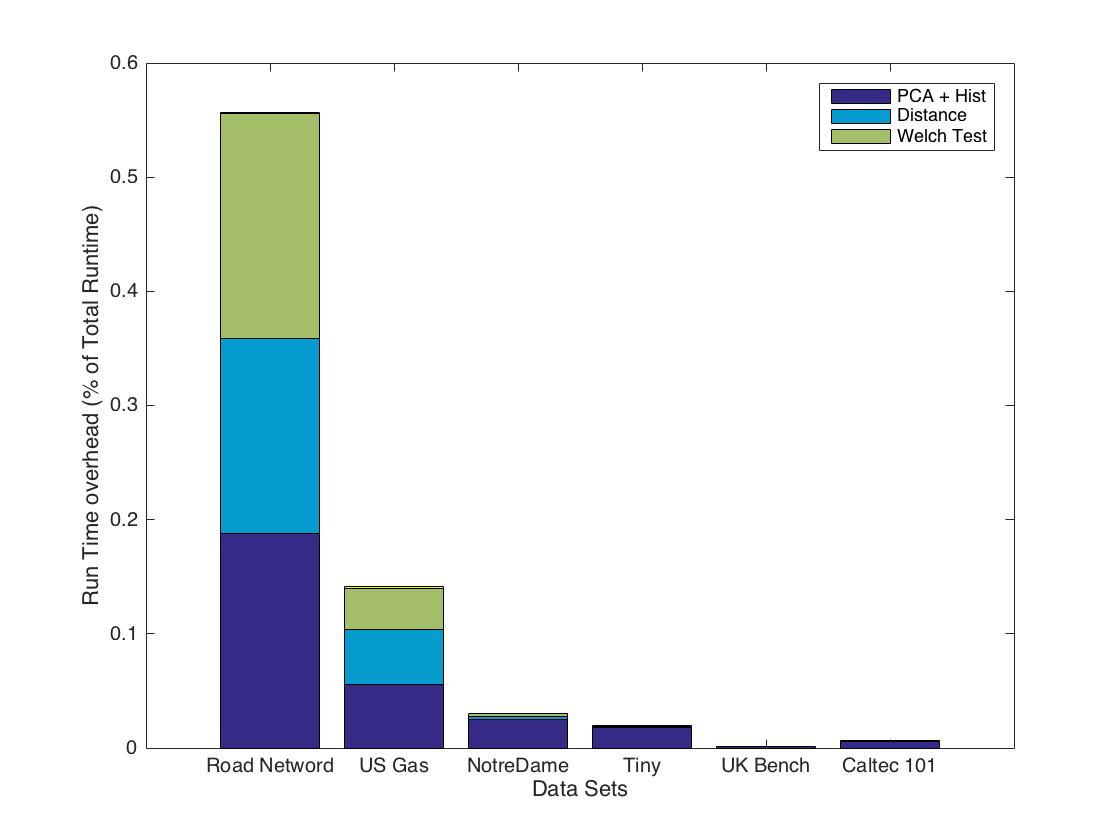
\includegraphics[width=\textwidth]{Chapter-5/figs/stacked_overhead}
    \caption{Best Match Selection Overhead (Maximum for Small \textit{k})}
    \centering
    \label{fig:selection_overhead}
\end{figure}

\begin{figure}[t!]
    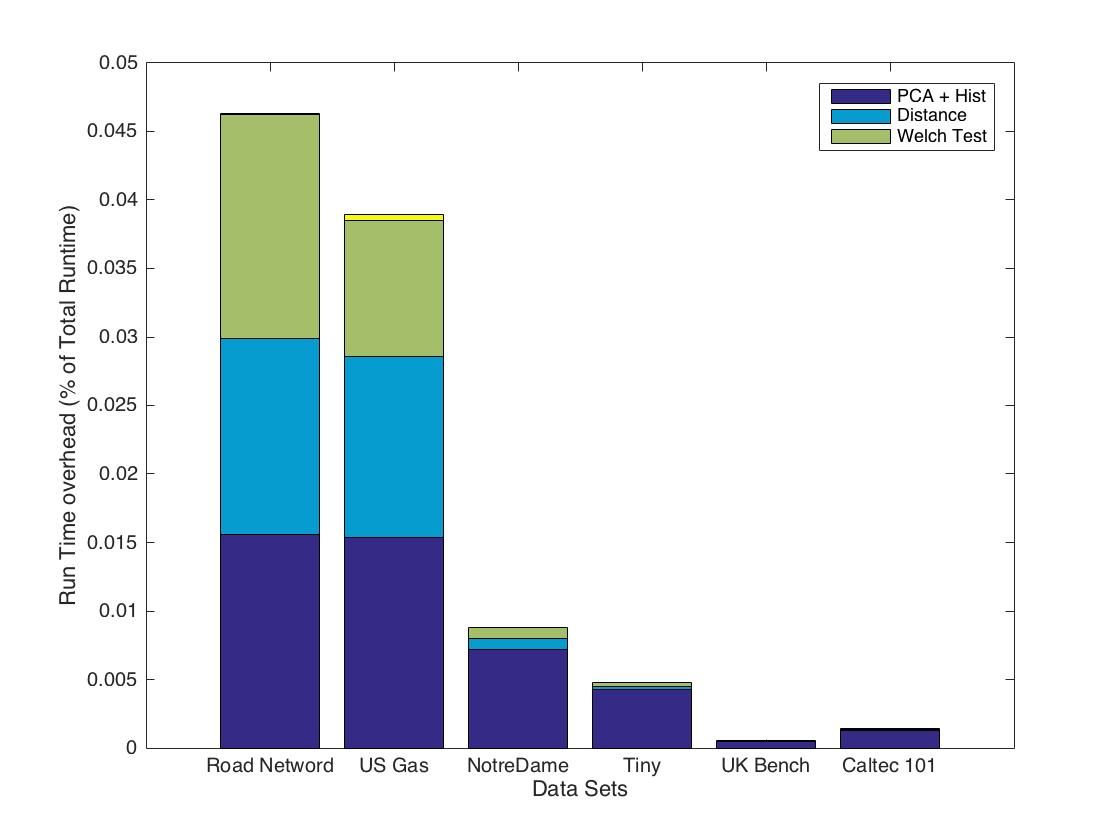
\includegraphics[width=\textwidth]{Chapter-5/figs/stacked_overhead_large}
    \caption{Best Match Selection Overhead (Minimum for Large \textit{k})}
    \centering
    \label{fig:selection_overhead_large}
\end{figure}

\begin{figure}[t!]
    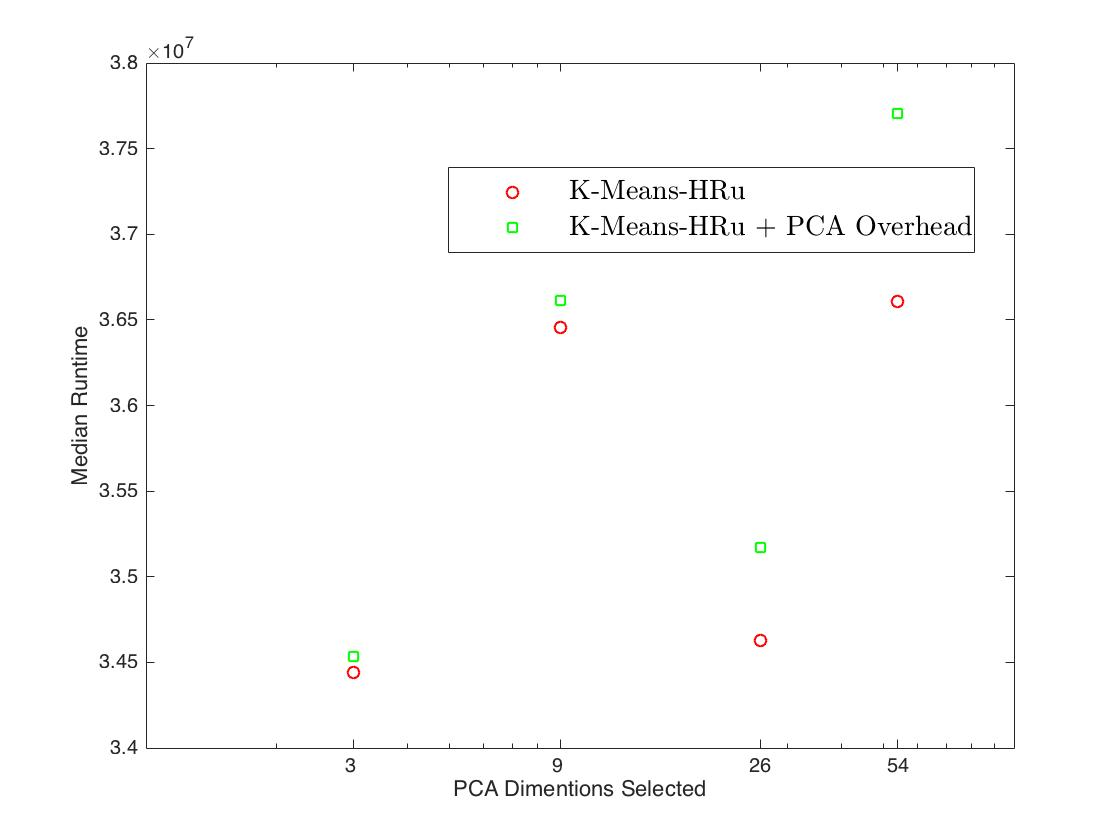
\includegraphics[width=\textwidth]{Chapter-5/figs/PCA_results}
    \caption{Performance for various PCA Dimension Count(Caltec 101; K = 600). Default PCA Dims: 3}
    \centering
    \label{fig:pca_overhead}
\end{figure}

Referencing the above mentioned tables and figures, we can also see that our selection mechanism takes only a very small percentage of the total run time for the algorithm for larger data sets (<~0.1\%) and while it may be a significant part of the initialization for smaller data sets the quality improvement in the initialization centroids is sufficient to offset the run time for the algorithm to be a viable initialization methodology for all data sets of varying sizes. 
Though speed up using our methodology is seen in all cases, it is best suited for larger data sets, as in that case our overhead for history best match selection almost becomes negligible.

From \textit{\textbf{Figure \ref{fig:pca_overhead}}} we can also see that even while retaining higher variances for historic data sets, no further speedup is seen in run time while the introduced overhead becomes a significant percentage for the total run time and may lead to further overheads as data set sizes increase.

\bgroup
\setlength{\arrayrulewidth}{0.2mm}
\setlength{\tabcolsep}{10pt}
\renewcommand{\arraystretch}{1}
\begin{table*}[t!]
\begin{minipage}{\textwidth}
\centering
%\begin{top}
\begin{tabular}{|l|c|c|c|c|c|c|r|}
\hline\hline
    \textbf{Data-set} & \textbf{n} & \textbf{d} & \textbf{k} & \textbf{K-Means (Time $\mu$S)} & \textbf{K-Means++} & \textbf{K-Means-HRU}\\
\hline\hline
    \textbf{Road Net.}   & 1.0E4 & 3 &
    \begin{tabular}{c} 40 \\ 80 \\ 120 \\ 240 \end{tabular} &
    \begin{tabular}{c} 8.5E4 \\ 1.6E5 \\ 2.01E5\\ 2.4E5\\ \end{tabular}&
    \begin{tabular}{c} 1.7X \\ 2.4X \\ 2.2X \\ 1.8X \\ \end{tabular} &
    \begin{tabular}{c} 6.7X \\ 10.0X \\ 10.0X \\1.6X \\ \end{tabular}\\
\hline
    \textbf{Kegg Net.}   & 2.0E4 & 10 &
    \begin{tabular}{c} 40 \\ 80 \\ 120 \\ 240 \end{tabular} &
    \begin{tabular}{c} 1.9E5 \\ 2.8E6 \\ 3.9E5 \\ 6.3E5 \\ \end{tabular} &
    \begin{tabular}{c}  2.5X \\ 1.9X \\ 1.6X \\ 1.9X \\ \end{tabular}&
    \begin{tabular}{c} 2X \\ 2.2X \\  2.8X \\ 3.2X \\ \end{tabular}\\
\hline
    \textbf{US Gas}   & 1.45E4 & 13 &
    \begin{tabular}{c} 40 \\ 80 \\ 120 \\ 240 \end{tabular} &
    \begin{tabular}{c} 3.2E5 \\ 4.7E5 \\ 5.2E5 \\ 8.9E5 \end{tabular} &
    \begin{tabular}{c} 2.4X \\ 1.9X \\ 1.9X \\ 1.7X \\  \end{tabular}&
    \begin{tabular}{c} 5.6X \\ 4.4X \\ 3.9X \\ 4.3X \\ \end{tabular}\\
\hline
    \textbf{NotreDame}   & 1.45E4 & 13 &
    \begin{tabular}{c} 40 \\ 80 \\ 120 \\ 240 \\ \end{tabular} &
    \begin{tabular}{c} 2.1E6 \\ 3.8E6 \\ 5.5E6 \\ 1.02E6\\ \end{tabular} &
    \begin{tabular}{c} 1.2X \\ 1.3X \\ 1.3X \\ 1.4X \\ \end{tabular}&
    \begin{tabular}{c} 2.4X \\ 2.3X \\ 2.3X \\ 2.3X \\ \end{tabular}\\
\hline
    \textbf{Tiny}   & 1.45E4 & 13 &
    \begin{tabular}{c} 80 \\ 120 \\ 240 \\ 360 \\ 480 \\ 600 \end{tabular} &
    \begin{tabular}{c} 0.9E8 \\ 1.3E8 \\ 2.5E8 \\ 3.2E8 \\ 3.9E8 \\ 4.3E8 \\ \end{tabular} &
    \begin{tabular}{c} 1.4X \\ 1.6X \\ 2.1X \\ 2.0X \\ 2.9X \\ 2.9X \\ \end{tabular}&
    \begin{tabular}{c} 2.8X \\ 2.9X \\ 3.8X \\ 2.7X \\ 4.1X \\ 4.1X \\  \end{tabular}\\
\hline
    \textbf{Uk Bench}   & 1.45E4 & 13 &
    \begin{tabular}{c} 80 \\ 120 \\ 240 \\ 360 \\ 480 \\ 600 \end{tabular} &
    \begin{tabular}{c} 1.7E7 \\ 2.3E7 \\ 4.2E7 \\ 4.7E7 \\ 5.8E7 \\ 6.8E7 \\ \end{tabular} &
    \begin{tabular}{c} 1.1X \\ 1.2X \\ 1.4X \\ 1.25X \\ 1.4X \\ 1.3X \\ \end{tabular}&
    \begin{tabular}{c} 2.7X \\ 2.5X \\ 2.5X \\ 2.4X \\ 2.1X \\ 2.3X \\ \end{tabular}\\
    
\hline
    \textbf{Caltec 101}   & 1.45E4 & 13 &
    \begin{tabular}{c} 80 \\ 120 \\ 240 \\ 360 \\ 480 \\ 600 \end{tabular} &
    \begin{tabular}{c} 1.9E7 \\ 2.2E7 \\ 4.2E7 \\ 5.3E7 \\ 6.5E7 \\ 7.3E7 \\ \end{tabular} &
    \begin{tabular}{c} 1.2X \\ 1.1X \\  1.4X \\ 1.4X \\   1.3X \\ 1.3X \\ \end{tabular}&
    \begin{tabular}{c} 2.6X \\ 2.1X \\ 2.3X \\ 2.3X \\ 2.2X \\ 2.1X \\ \end{tabular}\\
\hline
\end{tabular}
\caption{Runtime comparison: K-Means, K-Means++ and K-Means-HRU \textit{(*All times in $\mu$S)}}
\label{table:total_runtime_comparison}
%\end{top}
\end{minipage}
\end{table*}
\egroup

\textbf{Consistent Speed up for K-Means algorithm:} The end requirement of any initialization algorithm is to ensure that we achieve a consistent speed up over previous approaches. While running our initialization algorithm for K-Means we were able to see consistent speed up in run-time of algorithm as compared to both K-Means and K-Means++ algorithm for all data sets across a wide range of cluster counts ranging from 40 to 600. This is though dependent on quality of historical data sets available. A bad match may lead to relatively bad starting points which in turn leads to an increase in time taken for convergence. Not withstanding the above argument we were able to see consistently good performance by our algorithm for real data sets. This is largely due to the normalization of the data sets using the PCA based approach and then using cluster information based on this normalized data rather than the actual data. This also removes the need for the data to have Gaussian distribution. This gives a higher chance of finding a better historical match, thus giving consistent speed up over various data sets with different dimensionality\textit{(d)} and different cardinality\textit{(n)} for varying cluster counts \textit{k}.

Figures \ref{fig:box_speedup_small} and \ref{fig:box_speedup_large} shows the range of speed up across various data sets with varying degrees of freedom as well as different dimensionality for the same cluster counts. We can clearly see from the graphs that our algorithm consistently outperforms both the \textit{random K-Means(Lloyd’s Algorithm)} and the \textit{K-Means++ algorithm} in run time performance.


\begin{figure*}[p!]
    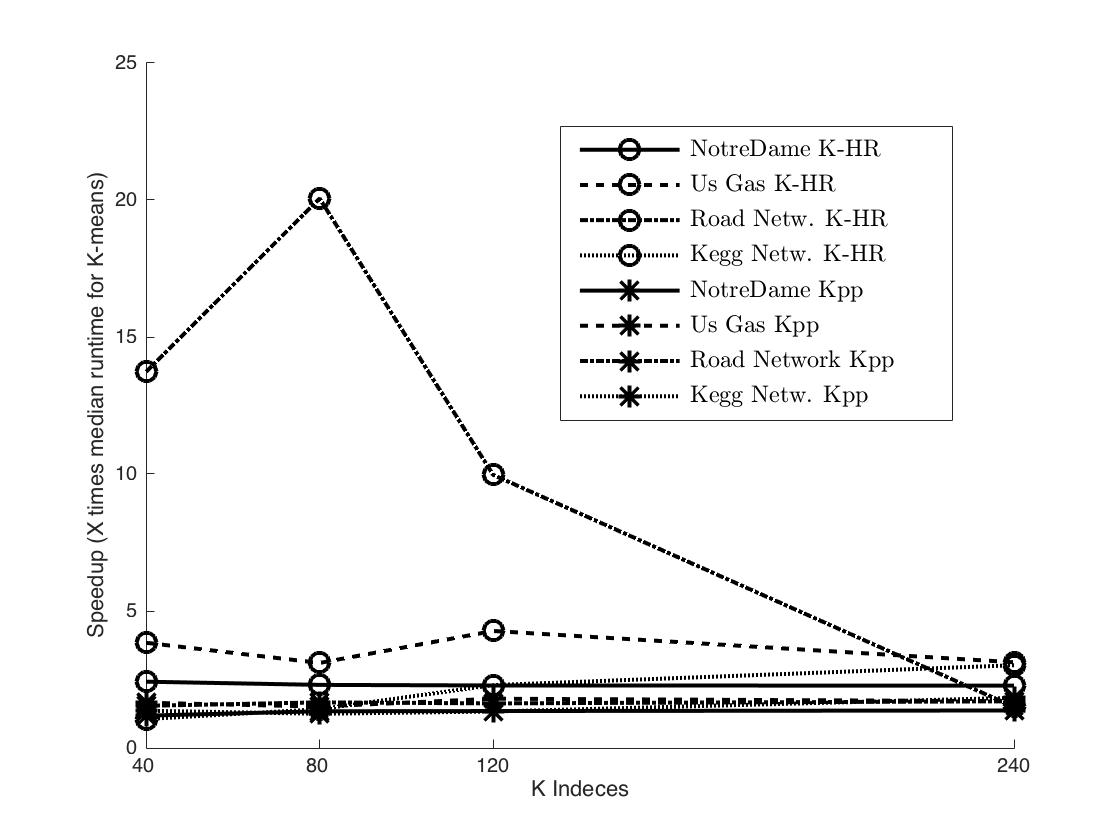
\includegraphics[width=\textwidth, height = 0.7\textheight, scale=1]{Chapter-5/figs/k_means_speedup_line_small}
    \caption{Median Speed up, Small Data (k=240)}
    \centering
    \label{fig:line_speedup_small}
\end{figure*}

\begin{figure*}[h!]
    \centering
        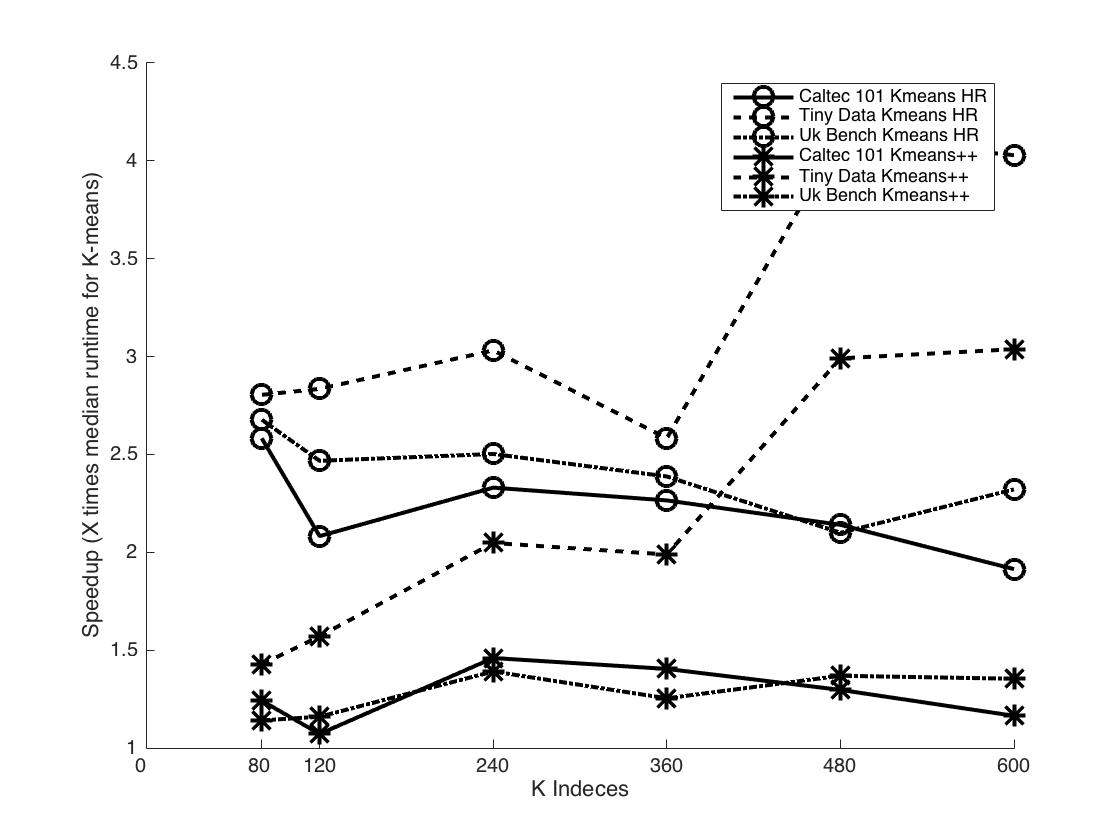
\includegraphics[width=\textwidth, height = 0.5\textheight, scale=1]{Chapter-5/figs/k_means_speedup_line_large}
    \caption{Median Speed up, Large Data (k=600)}
    \label{fig:line_speedup_large}
\end{figure*}

Figures \ref{fig:line_speedup_small} and \ref{fig:line_speedup_large} depict the speed up seen by our algorithm over various cluster sizes for all data sets. We can see that the general trend is that speed up seen is in general higher for larger cluster count. This is particularly true because as the cluster count increases we see a speed up in both the initialization method as well as the actual run time because of the improvement seen in the initialization centroids.

\setlength{\arrayrulewidth}{0.2mm}
\setlength{\tabcolsep}{10pt}
\renewcommand{\arraystretch}{1}
\begin{table*}[t!]
\begin{minipage}{\textwidth}
\centering
%\begin{top}
\begin{tabular}{|l|c|c|c|c|c|c|r|}
\hline\hline
    \textbf{Data-set} & \textbf{n} & \textbf{d} & \textbf{k} & \textbf{K-Means (Random)} & \textbf{K-Means++} & \textbf{K-Means-HRu}\\
\hline\hline
    \textbf{Road Net.}   & 1.0E4 & 3 &
    \begin{tabular}{c} 40 \\ 80 \\ 120 \\ 240 \end{tabular} &
    \begin{tabular}{c} 128 \\ 119 \\ 110 \\ 102 \\ \end{tabular}&
    \begin{tabular}{c} 69 \\ 52 \\ 46 \\ 79 \\ \end{tabular} &
    \begin{tabular}{c} 39 \\ 27 \\ 30 \\ 82 \\ \end{tabular}\\
\hline
    \textbf{US Gas}   & 1.45E4 & 13 &
    \begin{tabular}{c} 40 \\ 80 \\ 120 \\ 240 \end{tabular} &
    \begin{tabular}{c} 117 \\ 111 \\ 106 \\ 100 \\ \end{tabular} &
    \begin{tabular}{c} 58 \\ 59 \\ 58 \\ 55 \\ \end{tabular}&
    \begin{tabular}{c} 26 \\ 32 \\ 33 \\ 37\\ \end{tabular}\\
\hline
    \textbf{NotreDame}   & 1.45E4 & 13 &
    \begin{tabular}{c} 40 \\ 80 \\ 120 \\ 240 \\ \end{tabular} &
    \begin{tabular}{c} 162 \\ 154 \\ 132 \\ 103 \\ \end{tabular} &
    \begin{tabular}{c} 142 \\ 114.5 \\ 101 \\ 74 \\ \end{tabular}&
    \begin{tabular}{c} 69.5 \\ 65 \\ 60 \\ 48.5 \\ \end{tabular}\\
\hline
    \textbf{Tiny}   & 1.45E4 & 13 &
    \begin{tabular}{c} 80 \\ 120 \\ 240 \\ 360 \\ 480 \\ 600 \end{tabular} &
    \begin{tabular}{c} 195 \\ 181.5 \\ 168.5 \\ 129.5 \\ 119.5 \\ 111.5 \\ \end{tabular} &
    \begin{tabular}{c} 164 \\ 154.5 \\ 120.5 \\ 99.5 \\ 87.5 \\ 72 \\ \end{tabular}&
    \begin{tabular}{c} 108 \\ 98 \\ 87.5 \\ 74 \\ 67 \\ 58 \\ \end{tabular}\\
\hline
    \textbf{Uk Bench}   & 1.45E4 & 13 &
    \begin{tabular}{c} 80 \\ 120 \\ 240 \\ 360 \\ 480 \\ 600 \end{tabular} &
    \begin{tabular}{c} 274.5 \\ 273.5 \\ 251 \\ 233 \\ 216 \\ 196 \\ \end{tabular} &
    \begin{tabular}{c} 191 \\ 174.5 \\ 121 \\ 102 \\ 79.5 \\ 72 \\ \end{tabular}&
    \begin{tabular}{c} 85.5 \\ 82 \\ 75 \\ 70.5 \\ 63.5 \\ 57.5 \\ \end{tabular}\\
    
\hline
    \textbf{Caltec 101}   & 1.45E4 & 13 &
    \begin{tabular}{c} 80 \\ 120 \\ 240 \\ 360 \\ 480 \\ 600 \end{tabular} &
    \begin{tabular}{c} 219.5 \\ 171 \\ 178 \\ 146.5 \\ 137 \\ 108 \\ \end{tabular} &
    \begin{tabular}{c} 175.5 \\ 156.5 \\ 116.5 \\ 100 \\ 90 \\ 79 \\ \end{tabular}&
    \begin{tabular}{c} 84.5 \\ 80.5 \\ 74 \\ 69 \\ 61 \\ 58.5 \\ \end{tabular}\\
\hline
\end{tabular}
\caption{Median Iteration count comparison for K-Means, K-Means++ and K-Means with History Reuse.}
\label{table:iteration_comparison}
%\end{top}
\end{minipage}
\end{table*}

Results seen in Figures \ref{fig:selection_overhead} and \ref{fig:selection_overhead_large}  and Table \ref{table:total_runtime_comparison} together also show us that the speed ups are consistent irrespective of the cluster counts \textit{(k)} in terms of both the run time of the algorithms and the number of iterations taken for the convergence of the algorithm to similar error rate. This is again an intuitive results which confirms our hypothesis: a consistent selection methodology independent of the cluster index size would lead to sizable improvement in run time. This is so because run time improvement is seen in both the initialization overhead as well as the actual run time of the algorithm. As the cluster count\textit{(k)} increases, the amount of initialization overhead for both the above mentioned initialization methodology becomes a significant part of the total run time for the algorithm.

\begin{figure*}[t!]
    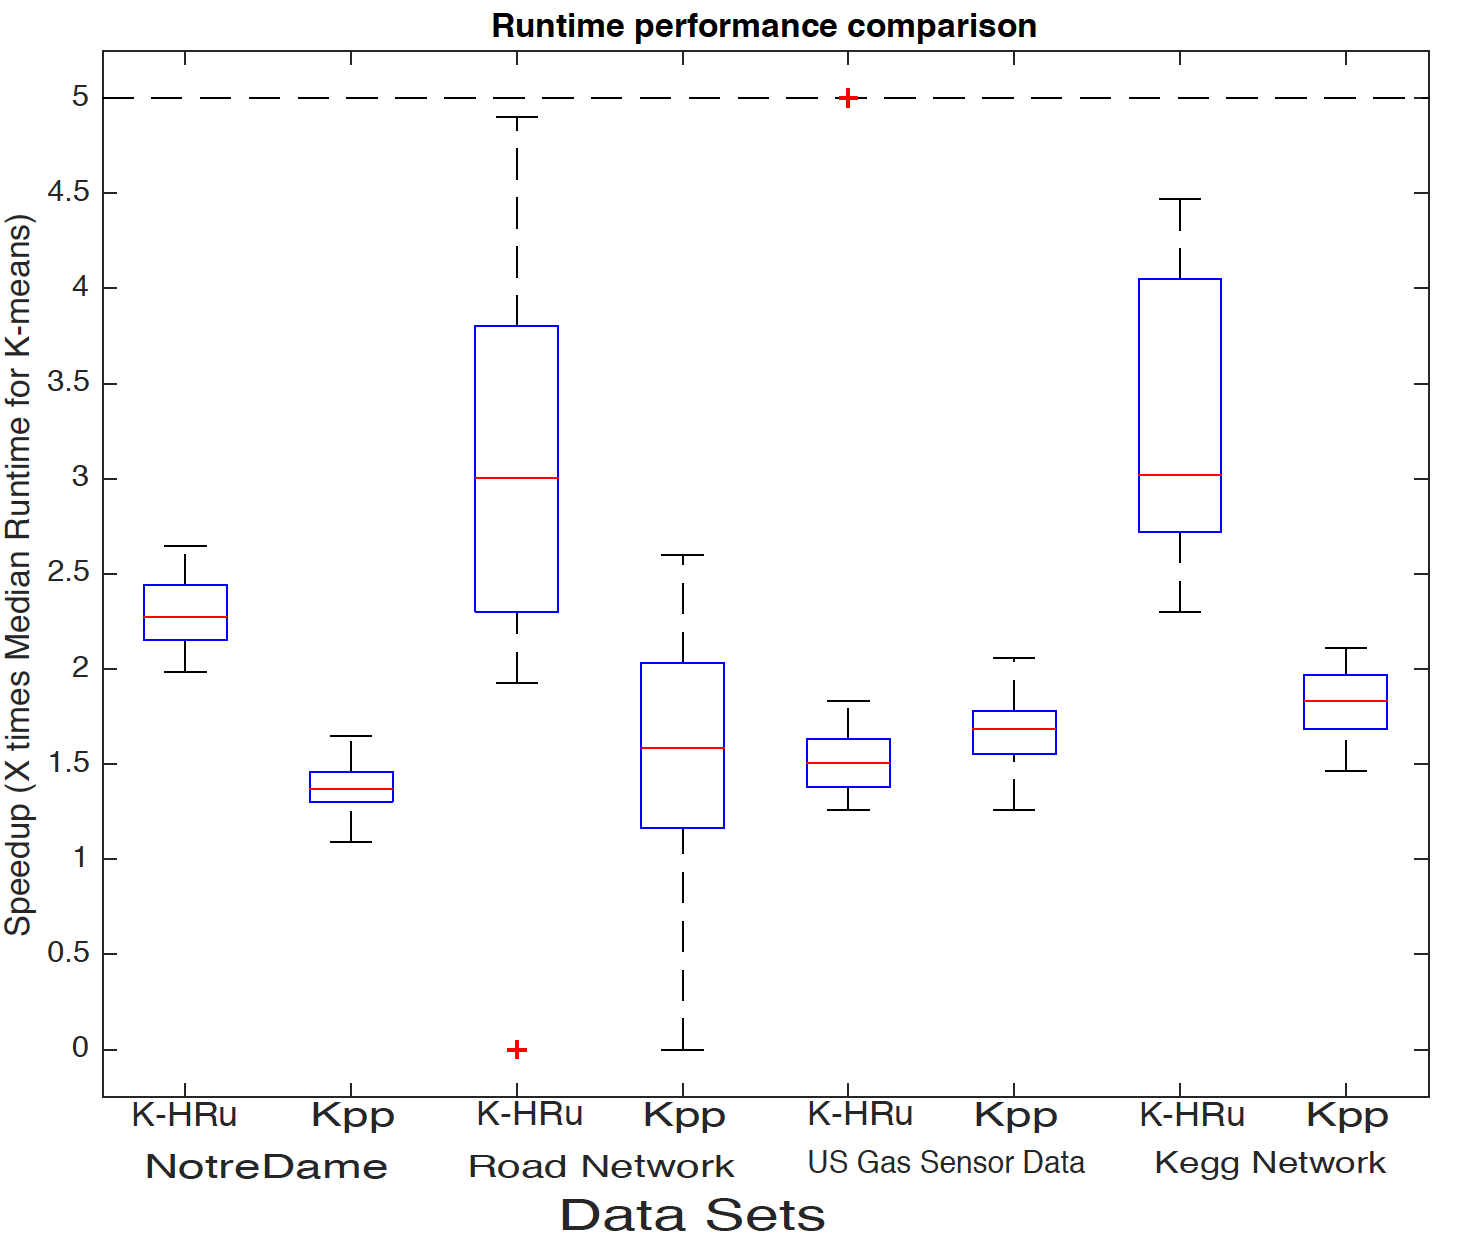
\includegraphics[width=\textwidth]{Chapter-5/figs/kpp+k_cust_speedup_small}
    \caption{Median Speed up, Small Data (k=240)(*K-HRu: K-Means-History Reuse; Kpp: K-Means++)}
    \centering
    \label{fig:box_speedup_small}
\end{figure*}

\begin{figure*}[b!]
    \centering
    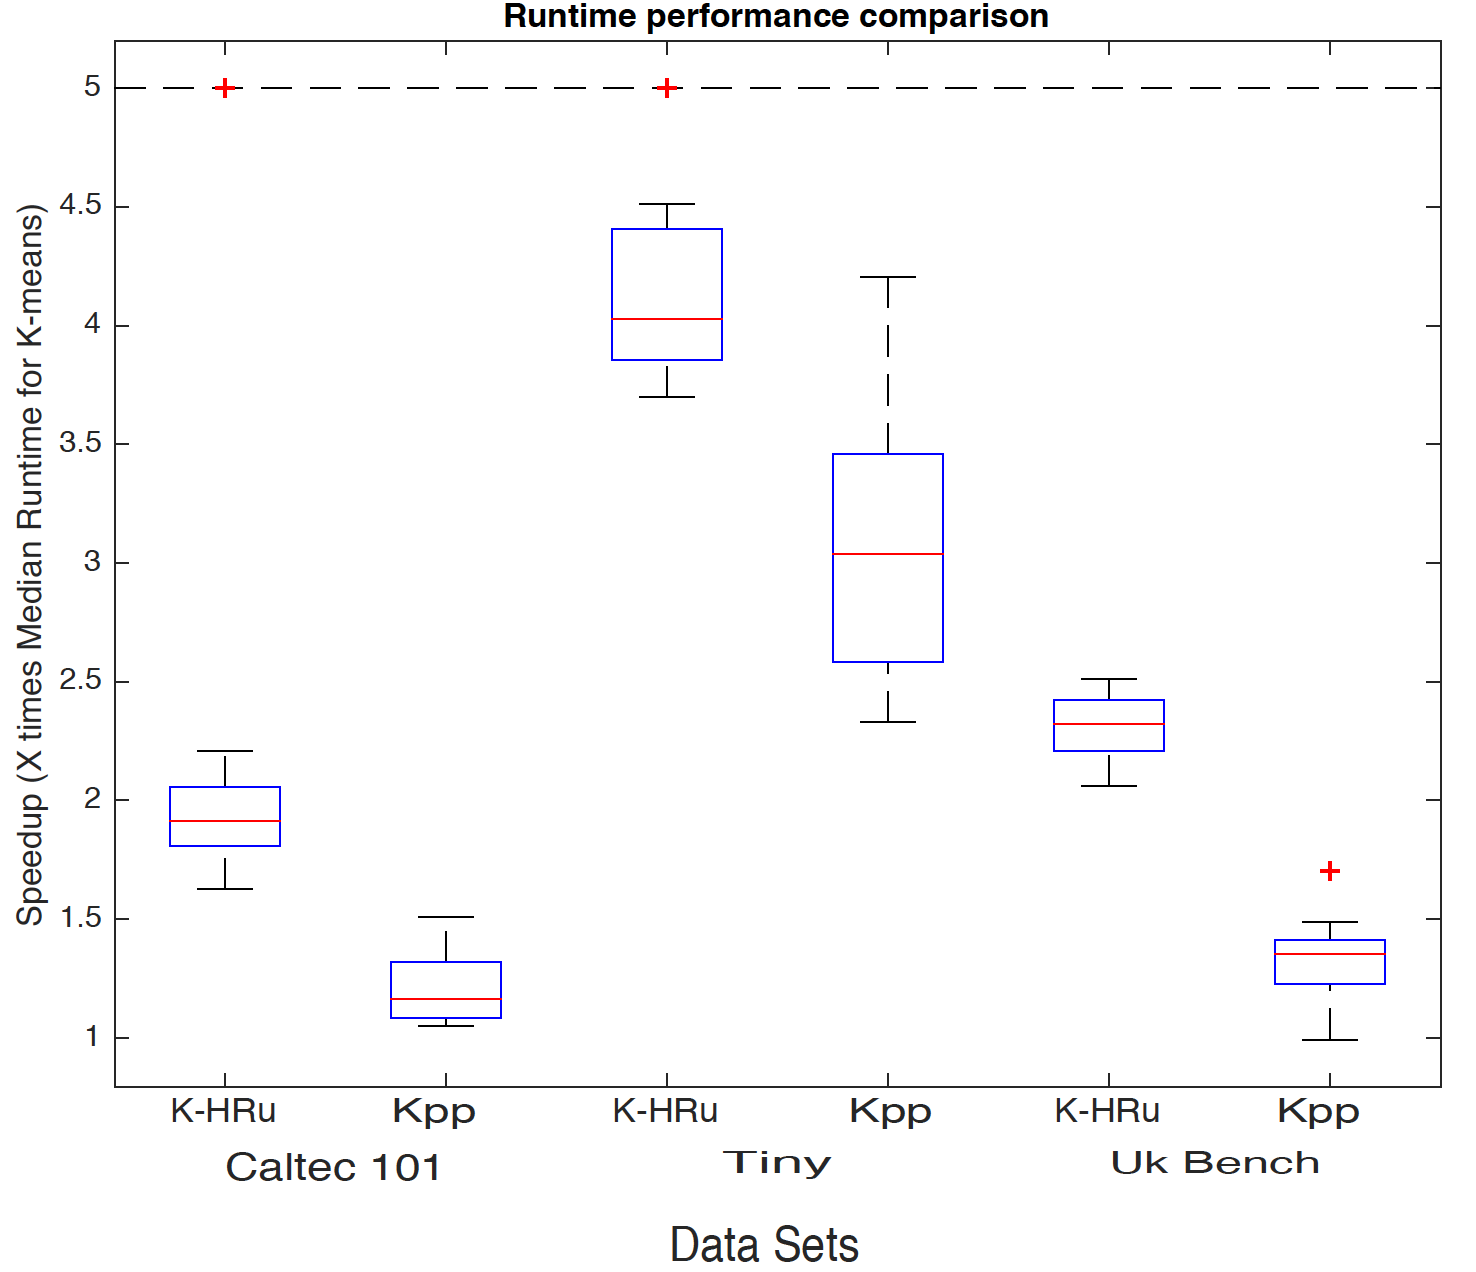
\includegraphics[width=\textwidth]{Chapter-5/figs/kcust+kpp_speedup_large}
    \caption{Median Speed up, Large Data (k=600)(*K-HRu: K-Means-History Reuse; Kpp: K-Means++)}
    \label{fig:box_speedup_large}
\end{figure*}

Another interesting feature seen in the above box plots is the varying degrees of speed up seen for the various segments for same data sets. Looking at the speed up that \textit{K-Means with History Reuse} achieves over the original \textit{K-Means (Lloyd’s algorithm)} we can see that the speed up is generally spread out over a larger range as compared to the performance of the \textit{K-Means++ algorithm} as compared to \textit{Lloyd’s Algorithm}. This thus, brings to fore our above made assumption about the quality of history data set available in terms of the probability of similarity . Our experiments prove our intuitive hypothesis that probabilistically similar data sets will tend to be classed together into similar clusters, thus making them the best history match data sets. The larger variance seen in the box plots above is testament to this. Normalization using \textit{PCA} of data sets, tends to mitigate this to a large extent thus providing us the ability to use history data not along same planes as well and thus providing a consistent speed up, but a better match of normalized data would provide even higher speed ups. We consistently saw that maximum speed ups are seen when the probability of similarity is higher. For segment with high probabilistic similarity we saw speed ups of up to and above \textit{\textbf{100 X}}.

\chapter{Future Work}
\label{chap-six}
As we have seen in our experimentation the speedup in the run time for the algorithm is dependent of the quality (probability of similarity) of historically available data sets for selection. Better quality selection would lead to better speedups. Thus one future work could involve new methodology for maintaining best quality history data sets.
Another possibility is to explore this History Reuse methodology for other algorithms. The general use of determining best match history data set is generic in nature (i.e. independent of the K-Means algorithm in itself) and thus can be extended to other algorithms such as the \textit{SVD based SVM algorithm}. Only a minor change to the training step specific to K-Means is required in such a case. This thus can be used to prove the comprehensible usability of this algorithm for all algorithms in the same class.
On the systems side the History reuse methodology can be used for memory data validation in Non Volatile Memory (NVM). This would prevent multiple expensive re-writes to NVM from main memory in case of already existing data.

Another area to explore may be the use of non uniform generation of hostogram for a better sample size selection in case of the screening algorithm. We chose not to explore this avenue in current work because our technique for unform buckets was showing significant performance gains. \cite{non_uniform_hist_1} shows an interesting way for generating non uniform histograms while still capturing sufficient desnity information such as to facilitate the selection of the density information more succinctly. Integral Histogram\cite{non_uniform_hist_2} represent a new a way of capturing non uniform histograms in the cartesian space and my be extended to our use as well. Both these above mentioned methods may help with furhter improving the accuracy of the screening algorithm.
\chapter{Conclusion}
\label{chap-seven}

In conclusion we would like to say that probabilistic metric for data-set comparison is
one of the best metrics for this purpose. It tells us the exact degree to which we can
expect the computation reuse to be successful for any historical data-set. It also represents a generic way of ranking data sets based on similarity and may have many more applications than just in history-reuse computation. We have also seen based on the above
results that the above mentioned algorithm is handy for all data sets irrespective if the dimensionality, cardinality or cluster count for the data set.
Though the algorithm shows speedups for all data sets for all cluster indexes we see a substantially higher speedup for larger cluster counts as this results in a speedup in both, the run time of the algorithm as well as the initialization step for the algorithm. The initialization is sped up considerably by our approach and this plays a vital part in the final speedup for larger cluster counts as initialization becomes a significant amount of the run time for both the \textit{Random K-Means} and the \textit{K-Means++} algorithm.
Since this can be used as a drop in replacement for any initialization method, it can be used with any flavour of the original K-Means Algorithm. It preserves the semantic of the original K-means. These appealing properties, plus its simplicity, make it a
practical replacement of the standard K-means as long as viable historical data sets are available for reuse.

%\restoregeometry


%%---------------------------------------------------------------------------%%
%%  Bibliography 

%%  You can use the bibitem list.
%\bibliographystyle{unsrt}
%\begin{%thebibliography}{99}
%\bibitem{cb02}
%Casella, G. and Berger, R.L. (2002)
%\newblock {\it Statistical Inference, Second Edition.}
%Duxbury Press, Belmont, CA.
%
%\bibitem{t06}
%Tsiatis, A.A. (2006)
%\newblock {\it Semiparametric Theory and Missing Data.}
%Springer, New York.
%
%\end{thebibliography}

%% or use BibTeX
%\bibliography{Ortiz-thesis}{}
%\bibliographystyle{plain}
%\nociterec{*}

%\bibliographystyle{plainnat}%plainnat is necessary to enable the use of citet. Natbib style file.
%\bibliography{Ortiz-thesis2}
%\ensureoddstart
\begin{spacing}{1}
 \setlength\bibitemsep{11pt} %22pt = 2*11pt, where fontsize is 11pt
 \addcontentsline{toc}{chapter}{{\uppercase{\bibname}}} %\textorpdfstring and \uppercase needed due to hyperref package http://www.latex-community.org/forum/viewtopic.php?f=44&t=16601
 %\vspace{-0.5in}
\titleformat{\chapter}[display]{\bf\filcenter
}{\chaptertitlename\ \thechapter}{11pt}{\bf\filcenter}
\titlespacing*{\chapter}{0pt}{-0.5in-9pt}{22pt}\printbibliography[heading=myheading]
\end{spacing}
%\bibliographystyle{apalike}


%%---------------------------------------------------------------------------%%
% Appendices
%\ensureoddstart
\restoregeometry
%\appendix
\newgeometry{margin=1in,lmargin=1.25in,footskip=\chapterfootskip, includehead, includefoot}


%\chapter{Lorem Ipsum}

\section{A First Section}

\paragraph{Filler Text} \lipsum[1-6]
%
\begin{figure}
  \centering
  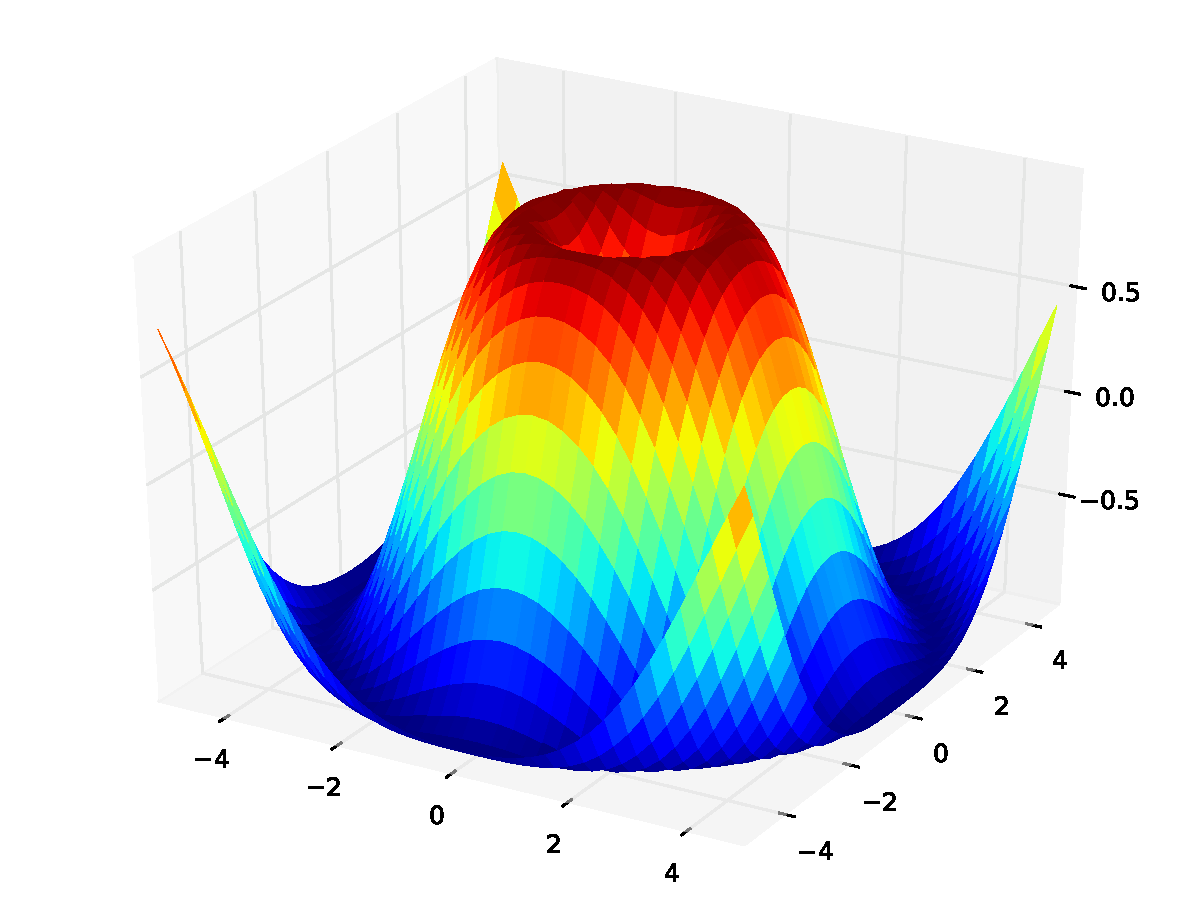
\includegraphics[width=0.6\textwidth]{Chapter-2/figs/threed}
  \caption{A figure in the appendix.}
  \label{fig:app}
\end{figure}
%
\lipsum[7-10]
\begin{table}
  \caption{A table in the appendix.}
  \label{tab:app}
  \begin{center}
    \begin{tabular}{lc}
      \toprule
      System & Author \\
      \midrule
      \TeX   & Donald Knuth   \\
      \LaTeX & Leslie Lamport \\
      \bottomrule
    \end{tabular}
  \end{center}
\end{table}
%

\section{A Second Section}

\lipsum[14-15]


\restoregeometry

%%---------------------------------------------------------------------------%%
%\ensureoddstart
\backmatter


\end{document}
